\documentclass[a4paper,12pt,oneside]{report}
\usepackage[utf8]{inputenc}
\usepackage[polish]{babel}
\usepackage[T1]{fontenc}
\usepackage{url}
\usepackage{graphicx}
\usepackage[a4paper,tmargin=4.5cm,rmargin=2.5cm,bmargin=2.5cm,lmargin=3.5cm,pdftex]{geometry}
\usepackage{setspace}
\usepackage{latexsym}
\usepackage{lscape}
% Dane o pracy
\author{Igor~Rzegocki}
\title{Migracja serwisu WWW z techniki PHP na Ruby~on~Rails}
\date{2008}
\pagestyle{headings}
\onehalfspacing

\begin{document}
\maketitle

% Dedykacja
\thispagestyle{empty}
\begin{flushright}
\vspace*{13cm}
\emph{Pracę swą dedykuję Grzegorzowi, którego nagła i niespodziewana śmierć pozostawiła ogromną pustkę w sercach jego przyjaciół}
\end{flushright}


\tableofcontents

\chapter{Wstęp}
\label{cha:wstep}

TODO

\chapter[Technologie po stronie serwera]{Technologie serwerowe wykorzystywane w aplikacjach internetowych}
\label{cha:serwer}

Ponieważ rynek aplikacji webowych jest dzisiaj duży, wielu producentów oprogramowania chce na nim zaistnieć. Dlatego prawie każdy język proponuje rozwiązania wspomagające budowę aplikacji internetowych. Najpopularniejszymi technologiami są C\#.NET, Java, Python, Ruby oraz PHP. Oczywiście nadal można wykorzystywać Perl czy C, ale dzisiaj mało kto wybiera te języki, ze względu na istnienie lepszych rozwiązań. Jeszcze 10 lat temu dużą uwagę zwracano na wydajność. Sprzęt komputerowy był stosunkowo drogi, więc sięgano do języków niskopoziomowych, które mogły zapewnić szybkie działanie przy małym zużyciu zasobów. Jednak dzisiaj sytuacja diametralnie się zmieniła. Oczywiście wydajność jest nadal ważna, ale zmiana serwera na szybszy lub dokupienie kolejnego aby przyspieszyć działanie aplikacji nie jest już tak relatywnie drogie. Na pierwszy plan wychodzą rozwiązania, które są wygodne dla programistów i pozwalają w krótkim czasie dodać nową funkcjonalność aplikacji lub zmodyfikować istniejącą. Obecnie niewielu programistów używa tylko standardowych bibliotek do budowy aplikacji. Każdy język oferuje dodatkowe biblioteki lub całe frameworki, które ułatwiają tworzenie i rozwój aplikacji. 

Poniżej zostały scharakteryzowane wyżej wymienione języki, oraz dostępne dla nich rozwiązania.

\section{Brama CGI}
\label{sec:cgi}
Na początku wszystkie strony internetowe były statyczne. To znaczy ich autorzy tworzyli osobny plik z kodem HTML dla każdej strony. Zmiana czegokolwiek wymagała manualnej edycji kodu. Oczywiście takich stron nie można nazwać aplikacją, bardziej pasujące byłoby tu określenie publikacja.

Przełomem w tworzeniu stron i początkiem aplikacji internetowych było stworzenie w 1993 specyfikacji interfejsu CGI.

,,CGI (ang. Common Gateway Interface, ) to znormalizowany interfejs, umożliwiający komunikację pomiędzy oprogramowaniem serwera WWW a innymi programami znajdującymi się na serwerze. Zazwyczaj program serwera WWW wysyła do przeglądarki statyczne dokumenty HTML. Za pomocą programów CGI można dynamicznie (na żądanie klienta) generować dokumenty HTML uzupełniając je np. treścią pobieraną z bazy danych.''\footnote{Źródło: \url{http://pl.wikipedia.org/wiki/CGI}}

CGI jest ogniwem, które łączy serwer WWW ze skryptem CGI. Zasada działania jest bardzo prosta. Serwer WWW dostarcza dane do programu poprzez standardowe wejście, lub pod postacią zmiennych środowiskowych. Program dostarcza swój wynik na standardowe wyjście, te dane natomiast są wysyłane przez serwer do przeglądarki. 

Dzięki temu, że po drugiej stronie bramy można umieścić program twórca serwisu jest w stanie dynamicznie generować dokumenty przed wysłaniem ich do przeglądarki. Jako źródło danych  może posłużyć baza danych, następnie te dane można sformatować aby były prezentowane w sposób czytelny w oknie przeglądarki. Jako parametry program może otrzymać dane z formularza, można generować przetwarzać i zapisywać dane z ankiet i kwestionariuszy. Można dynamicznie generować obrazy takie jak wykresy czy schematy.

Co najważniejsze implementacja CGI nie jest zależna od żadnej platformy, każdy serwer WWW może zaimplementować (i przeważnie implementuje) mechanizm CGI. Programy CGI można pisać w dowolnym języku programowania, wiele języków posiada biblioteki ułatwiające obsługę interfejsu. Standard CGI\footnote{Zobacz \url{http://www.w3.org/CGI/} i \url{http://hoohoo.ncsa.uiuc.edu/cgi/}} jest dostępny za darmo i nie zmienił się od 1995 roku. 

Początkowo językami najczęściej wykorzystywanymi do współpracy z CGI były Perl oraz C. Taki wybór był w pełni uzasadniony. C był i jest bardzo popularnym językiem programowania, a jego największą zaletą jest niewątpliwie wydajność. Natomiast Perl jest językiem stworzonym do przetwarzania danych tekstowych, więc znakomicie nadaje się do generowania kodu HTML.

Mechanizm bramy CGI jest wykorzystywany do dzisiaj, jednak nie jest to najszybsza metoda komunikacji pomiędzy serwerem WWW a aplikacją obsługującą żądania HTTP. CGI zastąpiły rozszerzenia dla serwerów dedykowane dla danego języka programowania, lub nawet całe serwery dedykowane.

\section{Java}
\label{sec:java}
Java jest darmową technologią rozwijaną pod kierunkiem firmy Sun Microsystems. Kod Javy jest kompilowany do tzw. bytecode’u, który następnie jest wykonywany przez maszynę wirtualną. Jej głównymi cechami są: pełna obiektowość,  niezależność od architektury (raz stworzony bytecode może być wykonywany na wirtualnej maszynie uruchomionej na dowolnym systemie operacyjnym), sieciowość i obsługa programowania rozproszonego, niezawodność i bezpieczeństwo.

Wczesne wersje Javy były krytykowane za powolne działanie, jednak dzisiejsze wersje są o wiele szybsze i bardzo stabilne. Do budowy aplikacji webowych Sun proponuje Serwlety wykonywane po stronie serwera , a także Aplety które mogą być osadzane na stronie WWW i wykonywane przez przeglądarkę na komputerze klienta. Jedną z alternatyw jest open sourceowy framework Struts\footnote{Zobacz \url{http://struts.apache.org/}}, wspomagany przez także open sourceową bibliotekę Hibernate\footnote{Zobacz \url{http://www.hibernate.org/}} ułatwiającą obsługę bazy danych. Popularny jest także framework Spring\footnote{Zobacz \url{http://www.springframework.org/}}. Java posiada także swój serwer WWW Tomcat\footnote{Zobacz \url{http://tomcat.apache.org/}}. Budowę aplikacji ułatwiają bardzo dobre zintegrowane środowiska programistyczne (IDE) Eclipse lub NetBeans dedykowane dla tego języka.

Dużą zaletą Javy jest to, że technologia ta ma bardzo dużo zastosowań. Można w niej tworzyć takie rozwiązania, jak aplikacje okienkowe czy nawet aplikacje dedykowane dla telefonów komórkowych. Posiada bardzo rozbudowane biblioteki obsługi sieci i oprogramowania rozproszonego. Java jest językiem kompleksowym jeżeli chodzi o możliwości zastosowania. Dlatego sprawdza się wszędzie tam gdzie jeden duży system, składający się z mniejszych aplikacji i ma za zadanie pełnić wiele ról przy jednoczesnej integracji. Taki przykładem może być system ERP IFS\footnote{Zobacz \url{http://www.ifsworld.com/pl/}}, który jest w całości napisany w Javie. Zarówno cała logika biznesowa, klient okienkowy przeznaczony dla stacji roboczych, jak i część webowa w której zrealizowany jest moduł zamówień dla klientów firmy.
\begin{itemize}
\item Plusy:
  \begin{itemize}
  \item stabilność i wydajność,
  \item cena (za darmo lub open source),
  \item międzyplatformowość,
  \item mnogość możliwych rozwiązań.
  \end{itemize}
\item Minusy:
  \begin{itemize}
  \item mnogość możliwych rozwiązań,
  \item potrzeba przekompilowania kodu po każdej zmianie,
  \item rozwój aplikacji w Javie jest stosunkowo pracochłonny.
  \end{itemize}
\end{itemize}

\section{C\#.NET}
\label{sec:dotnet}
C\# jest odpowiedzią firmy Microsoft na Javę Sun'a. Podobnie jak Java jest obiektowym językiem wysokopoziomowym, kompiluje się do języka Common Intermediate Language (CIL) (podobnie jak bytecode Javy), który następnie wykonywany jest w odpowiednim środowisku uruchomieniowym. Do budowy aplikacji webowych wykorzystuje się framework .NET\footnote{Zobacz \url{http://www.microsoft.com/net/}}. Framework .NET może współpracować również z innymi językami programowania takimi jak: Visual Basic, J\#, Jscript.Net, COBOL, Fortran, Lisp, Pyton, Perl i kilka innych. .NET ma o wiele większe możliwości niż tylko aplikacje webowe. Z powodzeniem może posłużyć do budowania aplikacji okienkowych dla systemu Windows. Dedykowany serwer WWW dla aplikacji .NET to IIS\footnote{Zobacz \url{http://www.iis.net/}}, oczywiście firmy Microsoft. Firma Microsoft dostarcza także środowisko programistyczne Visual Studio.

Podobnie jak Java, framework .NET z językiem C\#  ma także szersze spektrum zastosowań. Do znanych rozwiązań należy system obsługi banku PKO~BP~S.A. czy Getin~BANK~S.A zbudowane przez krakowską firmę Vsoft\footnote{Zobacz \url{http://www.vsoft.pl/}}. Obydwa systemy obsługują większą cześć procesów w banku i posiadają także moduł banokości internetowej. Dobrym przykładem zastosowań webowych jest serwis społecznościowy MySpace\footnote{Zobacz \url{http://www.myspace.com/}}, który posiada ponad 100 milionów użytkowników na całym świecie.
\begin{itemize}
\item Plusy:
  \begin{itemize}
  \item pełne wsparcie techniczne ze strony Microsoftu,
  \item sprawdzona i stabilna technologia.
  \end{itemize}
\item Minusy:
  \begin{itemize}
  \item cena,
  \item całkowita zależność od platformy Microsoft.
  \end{itemize}
\end{itemize}

\section{PHP}
\label{sec:php}
Język PHP\footnote{Zobacz \url{http://www.php.net/}} (ang. PHP: Hypertext Preprocessor, PHP: przetwornik hipertekstu) był od początku projektowany do wykorzystania na potrzeby aplikacji webowych. Pierwotnie PHP był raczej zestawem narzędzi niż językiem, dopiero od wersji 3 można mówić o języku programowania. PHP jest językiem interpretowanym, to znaczy przy każdym uruchomieniu interpreter czyta kod źródłowy i wykonuje go. Dzięki temu każda zmiana w aplikacji ma natychmiastowe skutki. Chociaż udostępnia on możliwość programowania obiektowego, tak naprawdę jest językiem proceduralnym. Jego popularność jest bardzo duża ze względu na łatwość jego użycia. Jest całkowicie darmowy (open source), a jego interpreter jest dostępny na wiele platform. Do PHP istnieje wiele frameworków (np. Zend Framework, Zoop Framework, Symfony, Prado, CakePHP etc.), wiele bibliotek do obsługi baz danych (np. ADOdb, Propel, PEAR::DB ect.). Jednak wydaje się, że PHP nie ma przed sobą przyszłości. 
\begin{itemize}
  \item jest wiele nieścisłości w nazwach funkcji i kolejności argumentów,
  \item część standardowych bibliotek jest udostępniana proceduralnie, a część obiektowo,
  \item kompatybilność wsteczna nie pozwala na uporządkowanie języka,
  \item brak możliwości obsługi niektórych błędów powoduje zatrzymanie wykonywania aplikacji
\end{itemize}
Skrypty PHP są serwowane najczęściej za pomocą serwera Apache2.

PHP jest bardzo popularne. Nadaje się zarówno do budowy dużych aplikacji (np. \url{http://www.yahoo.com/}, \url{http://www.interia.pl/}, \url{http://facebook.com} etc.), jak i do budowy małych komponentów (np. licznik odwiedzin, księga gości etc.). Jest on bardzo często pierwszym językiem od którego programiści zaczynają przygodę z aplikacjami webowymi.
\begin{itemize}
\item Plusy:
  \begin{itemize}
  \item łatwość użycia, 
  \item popularność,
  \item dostępność,
  \item cena (open source).
  \end{itemize}
\item Minusy:
  \begin{itemize}
  \item język proceduralny,
  \item brak perspektyw rozwoju,
  \item niespójne API (ang. Application Programming Interface)
  \end{itemize}
\end{itemize}

\section{Python}
\label{sec:python}
Python\footnote{Zobacz \url{http://python.org/}} to interpretowany język programowania stworzony jako następca języka ABC\footnote{Zobacz \url{http://idhub.com/abc/}}. Jest to język zaprojektowany z myślą o jak największej produktywności oraz o prostocie i czytelności kodu. Obsługuje też typy dynamiczne oraz automatyczne zarządzanie pamięcią. Ciekawą cechą Pythona jest to, że mimo iż różne części języka są opisane i ustandaryzowane, to język sam w sobie wciąż nie ma specyfikacji. 

Python jest językiem, który wspiera różne paradygmaty programowania:
\begin{itemize}
  \item Paradygmat programowania strukturalnego
  \item Paradygmat programowania funkcjonalnego
  \item Paradygmat programowanie obiektowego
\end{itemize}

Kolejną jego cechą jest rozszerzalność. Zamiast wbudowywać wszystko w rdzeń, można łatwo dokładać napisane w C lub C++ moduły. Dzięki temu sam środek języka pozostaje mały, elastyczny i wydajny. Takie rozwiązanie wzięło się z frustracji autora językiem ABC, w którym założenia były dokładnie odwrotne \footnote{Zobacz \url{http://www.artima.com/intv/pythonP.html}}.

Python bywa często wykorzystywany w aplikacjach internetowych. Najbardziej znana to \url{http://www.youtube.com/} a z polskich \url{http://www.grono.net/}. Doczekał się również wielu frameworków -- najpopularniejsze to Django\footnote{Zobacz \url{http://www.djangoproject.com/}}, Zope\footnote{Zobacz \url{http://www.zope.org/}}, TurboGears\footnote{Zobacz \url{http://www.turbogears.org/}} i Pylons\footnote{Zobacz \url{http://www.pylonshq.com/}}.

\begin{itemize}
  \item Plusy:
  \begin{itemize}
    \item elastyczność i rozszerzalność,
    \item wydajność,
    \item wiele frameworków.
  \end{itemize}
  \item Minusy:
  \begin{itemize}
    \item duża swoboda programowania powoduje bałagan w kodzie,
    \item wymóg stosowania wcięć znacznie utrudnia stworzenie dobrego systemu szablonów.
  \end{itemize}
\end{itemize}

\section{Ruby}
\label{sec:ror}
Ruby (dosł. rubin) to interpretowany, w pełni obiektowy język programowania stworzony w 1995 roku przez Yukihiro Matsumoto. Jak twierdzi jego autor\footnote{Porównaj http://www.informit.com/articles/article.aspx?p=18225\&rl=1} Ruby został zaprojektowany dla wydajności programistów, przy zachowaniu zasady dobrego interfejsu. Ze względu na pochodzenie języka (Japonia), początkowo był on mało popularny z powodu braku angielskiej dokumentacji. Jednak dzięki Internetowi rosła jego popularność i z czasem zaczęły się pojawiać artykuły w języku angielskim a wraz z nimi społeczność skupiona wokół tego języka. Przełomem była prezentacja w 2003 roku frameworku Ruby On Rails (dosł. rubin na szynach). Rails posiadają wszystko co jest niezbędne do budowy aplikacji webowych i znakomicie nadają się do bardzo szybkiej budowy małych aplikacji a także budowania prototypów aplikacji. Interpretery Rubiego istnieją na każdą platformę. Jedyną wadą języka zdaje się być jego wydajność (podobnie jak we wczesnych wersjach Javy), którą jednak można zwiększyć wykorzystując JRuby (implementację interpretera w języku Java). Ruby posiada swoje dwa serwery WWW -- Mongrel oraz Webrick, można używać także serwera Apache za pośrednictwem CGI lub rozszerzenia mod\_ruby.

\begin{itemize}
\item Plusy:
  \begin{itemize}
  \item darmowy
  \item pełna obiektowość
  \item duże perspektywy rozwoju, 
  \item przejrzystość kodu, 
  \item bardzo prosty w nauce
  \item duża aktywna społeczność zawsze chętna do pomocy 
  \item pisanie w Rubym to naprawdę świetna zabawa
  \end{itemize}
\item Minusy:
  \begin{itemize}
  \item niska wydajność
  \item brak znanych udanych wdrożeń
  \end{itemize}
\end{itemize}

\section{Ruby on Rails}
\label{sec:ror}

Współdziałanie frameworka Rails i języka Ruby ma umożliwiać programiście szybkie, wydajne i bezbolesne tworzenie aplikacji internetowych. Efekt taki uzyskano łącząc cechy dynamicznego i obiektowego języka ze sprawdzonymi wzorcami i schematami dotyczącymi projektowania aplikacji internetowych.

,,Często ludzie, zwłaszcza inżynierowie oprogramowania skupiają się na maszynach. Sądzą oni iż robiąc to tak sprawimy, iż maszyna będzie pracowała szybciej. Jeśli znów zmienimy coś innego to znów maszyna przyśpieszy. Skupiają się tylko na procesorach i wydajności. Tak naprawdę potrzebujemy skupić się na programistach. Na tym jak ludzie chcą aby ich aplikacje były zaprojektowane i jak działały. To my jesteśmy władcami. One są niewolnikami.”\footnote{Yukihiro Matsumoto, The Philosophy of Ruby, 2003}. Słowa te najlepiej obrazują filozofię języka jak i to co można uzyskać używając połączonych sił Ruby i Rails. 

\begin{itemize}
  \item Szybkość, łatwość i przyjemność z pisania,
  \item Reguła DRY (zob. rozdz.~\ref{sec:dry}, str.~\pageref{sec:dry}),
  \item Reguła Convention over Configuration (zob. rozdz.~\ref{sec:coc}, str.~\pageref{sec:coc}),
  \item Architektura MVC jako sprawdzony wzorzec budowania aplikacji internetowych (zob. rozdz.~\ref{sec:mvc}, str.~\pageref{sec:mvc}),
  \item Integralną częścią aplikacji są wszelakie testy, które pomagają i automatyzują proces wyszukiwania błędów,
  \item Prostota w dodawaniu wtyczek, które rozszerzają aplikację o całą gamę gotowych funkcjonalności od prostego logowania do całych modułów zarządzających.
\end{itemize}

Framework Rails zbudowany jest z trzech zasadniczych elementów:

\begin{itemize}
\item \emph{Active Record} -- mechanizm ORM (zob. rozdz.~\ref{sec:orm}, str.~\pageref{sec:orm}) odpowiada za odwzorowanie obiektowej architektury obiektów na relacyjną strukturę bazy danych. Różni się on od zwyczajnych systemów ORM minimalizacją potrzebnych konfiguracji ze strony programisty. Jednocześnie jest bardzo potężnym narzędziem. Odpowiada za generowanie modeli czyli za literkę „M” w MVC.
\item \emph{Action Pack} -- w którego skład wchodzą klasy obsługujące widoki (literka „V” w MVC) oraz kontrolery (literka „C” w MVC). Dzięki uniwersalnemu podejściu widoki nie muszą tylko i wyłącznie ograniczać się do produkowania kodu HTML który potem wyświetlany jest w przeglądarce. W bardzo prosty sposób możemy przekształcać nasze widoki do XML’a , generować dynamiczny JavaScript , używać protokołu SOAP oraz wiele innych. Kontrolery natomiast są logiką całej naszej aplikacji. Zarządzają interakcjami między użytkownikami a systemem, modelami a widokami itd.
\item Mechanizm ,,scaffolding'' -- służy bardzo szybkiemu tworzeniu gotowych powiązań między modelem a kontrolerem a widokami. W praktyce jest to po prostu generator gotowego kodu źródłowego dla danego modelu. Tworzone są wszystkie podstawowe akcje jak stwórz, czytaj, edytuj, kasuj (zob. rozdz.~\ref{sec:crud}, str.~\pageref{sec:crud}). Zwalnia to programistę z pisania po raz setny tych samych wspólnych zachowań dla modelu i pozwala skupić się na tym jak aplikacja ma działać a nie na wymyślaniu kolejnego systemu walidacji danych.
\end{itemize}

Kolejnym ważnym elementem przemawiającym za, jest ilość dostępnych darmowych wtyczek które automatyzują/ułatwiają wykonywanie określonych zadań. Główny serwis http://rubyforge.org który zajmuje się zbieraniem i informowaniem o wtyczkach posiada obecnie 5912\footnote{Stan na 24 maja 2008 r.} różnych wtyczek które możemy użyć w naszym projekcie.

W używaniu Ruby~on~Rails jest coś magicznego, coś co bardzo ciężko opisać czy poczuć przy pierwszym zetknięciu się. Najprościej można powiedzieć, że to po prostu działa i jest zrobione tak jak powinno. Wszystko ma swoje określone miejsce, zachowanie i działa dokładnie tak jak tego oczekujemy.

Dzięki uniwersalności i prostocie możemy stosować połączenie Ruby~on~Rails wszędzie tam gdzie potrzebujemy szybko, przyjemnie i bezproblemowo stworzyć aplikację internetową. W bardzo krótkim czasie możemy stworzyć gotowe elementy naszego systemu. Każdy kawałek kodu ma swoje jedno dokładnie pasujące miejsce i nawet tworząc tylko podstawowy szkielet aplikacji mamy już bardzo dużo rzeczy zrobionych za nas, czekających tylko do wykorzystania.

Największą aplikacja napisaną całkowicie w technologii Ruby~on~Rails jest Basecamp\footnote{Zobacz http://www.basecamphq.com/}. Basecamp jest aplikacją wspomagającą zarządzanie projektami, która obecnie obsługuje ponad milion użytkowników. Drugą duża aplikacją jest Twitter\footnote{Zobacz http://www.twitter.com/}. Twitter jest z kolei platformą służącą do ,,mikroblogowania'' (czyli pisania wpisów nie dłuższych niż 140 znaków). Obecnie cała społeczność Ruby~on~Rails śledzi z zapartym tchem dzieje Twittera, gdyż ma on ogromne problemy wydajnościowe. Od tego jak je rozwiąże, zależy jak inwestorzy komercyjni ocenią przydatność samego frameworka.

\chapter[Technologie po stronie klienta]{Technologie po stronie klienta wykorzystywane w aplikacjach internetowych}
\label{cha:klient}

\section{HTTP}
\label{sec:http}
,,HTTP (HyperText Transfer Protocol - protokół przesyłania dokumentów hypertekstowych) to protokół sieci WWW. Obecną definicję HTTP stanowi RFC~2616. Za pomocą protokołu HTTP przesyła się żądania udostępnienia dokumentów WWW, informacje o kliknięciu odnośnika oraz informacje z formularzy. Zadaniem stron WWW jest publikowanie informacji - natomiast protokół HTTP właśnie to umożliwia.''\footnote{Źródło: \url{http://pl.wikipedia.org/wiki/HTTP}}

HTTP jest to protokół zapytań i odpowiedzi pomiędzy klientem a serwerem. Jest on bardzo użyteczny, ponieważ udostępnia znormalizowany sposób komunikowania się komputerów ze sobą. Określa on formę żądań klienta dotyczących danych oraz formę odpowiedzi serwera na te żądania. Jest to protokół bezstanowy ponieważ nie zachowuje żadnych informacji o poprzednich transakcjach z klientem. Protokół definiuje osiem metod, które mogą być użyte w żądaniu HTTP:
\begin{itemize}
  \item \emph{GET} - pobranie informacji wskazanej przez URL (ang. Uniform Resource Locator, jednoznaczny wskaźnik zasobu),
  \item \emph{HEAD} - pobiera informacje o tym czy dana informacja istnieje
  \item \emph{PUT} - informacja potwierdzająca pobranie danych w postaci pliku od klienta przez serwer
  \item \emph{POST} - analogicznie jak powyżej tyle, że informacja nie musi być plikiem (np. formularze)
  \item \emph{DELETE} - żądanie usunięcia informacji -- wymagane odpowiednie uprawnienia
  \item \emph{OPTIONS} - informacje o opcjach i wymaganiach istniejących w kanale komunikacyjnym, 
  \item \emph{TRACE} - analiza i diagnostyka kanału komunikacyjnego, 
  \item \emph{CONNECT} - żądanie wykorzystywane w tunelujących serwerach proxy.
\end{itemize}

Na potrzeby przeglądania stron WWW używane są metody GET oraz POST. Natomiast cały zestaw metod protokołu daje znacznie większe możliwości i może posłużyć do kompleksowej wymiany informacji pomiędzy komputerami w sieci Internet.

\section{HTML}
\label{sec:html}
Zawartość strony internetowej jest hipertekstem, znaczy to, że użytkownik oglądając stronę internetową może podążać za hiperłączami, które przenoszą go do innych stron internetowych w ramach tego samego serwera internetowego lub innych dostępnych w ramach sieci.

,,Hipertekst to organizacja danych w postaci niezależnych leksji połączonych hiperłączami. Hipertekst cechuje nielinearność i niestrukturalność układu leksji. Oznacza to, że nie ma z góry zdefiniowanej kolejności czytania leksji, a nawigacja między nimi zależy wyłącznie od użytkownika.''\footnote{Źródło \url{http://pl.wikipedia.org/wiki/Hipertekst}}

Implementacją hipertekstu na potrzeby WWW jest język HTML 

,,HTML (HyperText Markup Language, hipertekstowy język znaczników), to język składający się ze znaczników oraz reguł ich poprawnego stosowania (gramatyki, semantyki), stosowany do pisania stron WWW. HTML jest teoretycznie aplikacją SGML, tzn. został zdefiniowany za pomocą SGML, będącego tzw. metajęzykiem (językiem służącym do definiowania innych języków).''\footnote{Źródło \url{http://pl.wikipedia.org/wiki/HTML}}

Wraz z rozwojem sieci WWW pojawiła się potrzeba rozwoju języka HTML aby posiadał on możliwość dołączania do testów danych tabelarycznych grafik czy plików multimedialnych. Kolejne wersje języka rozwijane były niezależnie przez producentów przeglądarek internetowych, co doprowadziło do częściowej  niekompatybilności wersji HTML zaimplementowanych w przeglądarkach różnych producentów. Próbą odpowiedzi na tę sytuację było stworzenie W3C\footnote{Zobacz \url{http://www.w3c.org/}} czyli World Wide Web Consortium, organizacji, która zajmuje się ustanawianiem wspólnych standardów HTML, a także innych spraw związanych z pisaniem stron WWW. Ostatnią wersją HTML jest wersja 4.01, która próbuje wydzielić zarządzanie wyglądem strony do kaskadowych arkuszy stylów (CSS). Na jakiś czas W3C zaprzestało rozwoju HTML i postanowiło dostosować język do XML (ang. eXtensible Markup Language). W wyniku powstał XHTML, dla którego istnieje tryb zgodności z HTML, który to umożliwia wyświetlenie kodu XHTML w przeglądarkach zgodnych z HTML 4.01. Zmiana ta ma zapewnić większą rozszerzalność i dostępność języka. Z tego powodu właśnie XHTML jest obecnie zalecanym standardem tworzenia stron WWW. Obecną najnowszą wersją hipertekstu na potrzeby stron WWW jest XHTML 1.1\footnote{Zobacz \url{http://www.w3.org/TR/xhtml11/}}, a dla niego arkusze styli CSS 2.1\footnote{Zobacz \url{http://www.w3.org/TR/REC-CSS2/}}. Kolejną wersją języka (X)HTML miał być XHTML 2.0, jednak ta droga rozwoju została ostatecznie uznana za nietrafioną i rozwój XHTML 2.0 został zarzucony na rzecz HTML 5\footnote{Zobacz \url{http://www.w3.org/html/wg/html5/}}, nad rozwojem którego trwają obecnie intensywne prace.

\section{CSS}
\label{sec:css}
,,Kaskadowe arkusze stylów (ang. Cascading Style Sheets, CSS) to język służący do opisu formy prezentacji (wyświetlania) stron WWW. CSS został opracowany przez organizację W3C w 1996 r. jako potomek języka DSSSL przeznaczony do używania w połączeniu z SGML-em. Pierwszy szkic CSS zaproponował w 1994 r. Håkon Wium Lie.\footnote{Zobacz http://www.w3.org/People/howcome/p/cascade.html}''

CSS jest wykorzystywany aby wspomóc czytniki stron WWW w definiowaniu kolorów, czcionek, układów i innych aspektów prezentacji dokumentu. Głównym założeniem projektowym była separacja warstwy treści (zapisanej w HTML albo w podobnym języku znaczników) od warstwy prezentacji (zapisanej w CSS). Taka separacja znacznie podnosi dostępność treści, zapewnia dużo większą elastyczność i kontrolę nad aspektami prezentacyjnymi dokumentu. Dodatkowo redukuje powtarzalność w warstwie dokumentu (jeżeli chcemy np. aby wszystkie nagłówki były koloru zielonego, nie musimy go nadawać każdemu z nich z osobna). CSS pozwala również na to, aby ta sama treść była wyświetlana w różny sposób na różnych urządzeniach (np. inaczej będziemy wyświetlać stronę na ekranie komputera, inaczej na telefonie komórkowym a jeszcze inaczej w wersji do druki). CSS określa też priorytety z jakimi należy nakładać kolejne właściwości. Najnowszą wersją CSS jest obecnia wersja 2.1 -- trwają jednak prace, nad wersją trzecią\footnote{Zobacz \url{http://www.w3.org/Style/CSS/current-work}}.

\section{JavaScript}
\label{sec:javascript}
JavaScript jest skryptowym językiem programowania, który został opracowany przez firmę Netscape na potrzeby stron internetowych. JavaScript jest wersją standaryzowanego języka ECMAScript\footnote{Pełny standard \url{http://www.ecma-international.org/publications/files/ECMA-ST/Ecma-262.pdf}}.

Nazwa nasuwa skojarzenie z językiem Java, jednak oba języki nie mają ze sobą wiele wspólnego, oprócz tego że ich składnia jest zaczerpnięta z języka C. W połączeniu z Document Object Model\footnote{Zobacz \url{http://www.w3.org/DOM/}} JavaScript stał się o wiele bardziej potężną technologią niż przewidywali jej twórcy. Po załadowaniu strony programista ma możliwość manipulacji strukturą dokumentu (załadowanej do przeglądarki strony), może także tworzyć funkcje, które reagują na zdarzenia występujące w oknie przeglądarki (ruchy, klikniecie myszką, naciśnięcie klawisza na klawiaturze etc.). Połączenie HTML ze skryptami języka JavaScript nazywane jest Dynamic HTML (DHTML), czyli dynamiczny HTML, aby uwydatnić różnicę ze statycznymi stronami HTML. 
Przełomem w DHTML było udostępnienie obiektu XMLHttpRequest (XHR). XHR umożliwia wysyłanie żądań HTTP z poziomu języka JavaScript już po załadowaniu się strony internetowej w trakcie interakcji z użytkownikiem. Otrzymane odpowiedzi serwera są wówczas wykorzystywane do modyfikacji załadowanego dokumentu. Możliwość asynchronicznego wykonywania żądań sprawia, że są one wykonywane w tle i nie przerywają interakcji użytkownika ze stroną, dynamicznie ją zmieniając. Technika wykorzystania obiektu XHR została nazwana AJAX (ang. Asynchronous JavaScript and XML, asynchroniczny JavaScript i XML) . Dzisiaj każda przeglądarka udostępnia XHR. AJAX sprawdza się tam gdzie nie ma potrzeby przeładowywania całej strony, a tylko jej części lub gdzie w ogóle nie trzeba dokonywać przeładowania a jedynie wysłać informację do serwera WWW. AJAX oszczędza czas użytkownika (w trakcie doładowywania informacji może on przeglądać stronę, która dalej jest dla niego dostępna) oraz zmniejsza obciążenie serwera (doładowywanie tylko części informacji zamiast całej strony ogranicza ilość danych wysyłanych do przeglądarki). 

\section{RSS}
\label{sec:rss}
RSS (ang. Really Simple Syndication, bardzo proste rozpowszechnianie artykułów) jest to format języków znacznikowych używany do publikowania często zmieniającej się treści, takiej jak wpisy na blogach, nagłówki wiadomości, podcasty etc. Dokument RSS zawiera zazwyczaj podsumowanie przypisanej mu strony WWW lub jej pełną zawartość. 

RSS umożliwia ludziom, bycie na bieżąco ze stronami internetowymi dzięki automatycznym programom zwanymi ,,czytnikami RSS''. Aplikacje te, zbierają wiadomości z witryn wybranych przez użytkownika, a następnie przedstawiają w skondensowanej i przystępnej formie. Dzięki temu, nie ma potrzeby odwiedzania każdej witryny -- wszystkie można przeglądać z poziomu jednej aplikacji. Oznacza to więc znaczną oszczędność czasu. Zasada działania agregatora RSS jest prosta. Co jakiś czas (aplikacja działająca w tle, lub agregator internetowy\footnote{Na przykład \url{http://reader.google.com/}}) lub przy każdym uruchomieniu następuje sprawdzenie wszystkich wpisanych kanałów RSS, pod kątem nowej zawartości. Jeśli zostanie odnaleziona, następuje jej ściągnięcie i oznaczenie jako nieprzeczytana. 

Oczywiście wiadomość RSS nie jest w żaden sposób ograniczona w stosunku do normalnej strony WWW. Z racji tego, że jest to zwykły plik XML, może zawierać odnośniki, grafikę a nawet informacje multimedialne. Każda wiadomość RSS zawiera także hiperlink do oryginału (co jest istotne w przypadku skrótów). 

Wyróżnia się następujące ,,rodziny'' RSS:
\begin{itemize}
  \item Really Simple Syndication (RSS 2.0)
  \item RDF Site Summary (RSS 1.0 i RSS 0.90)
  \item Rich Site Summary (RSS 0.91).
\end{itemize}

\section{YAML}
\label{sec:yaml}
YAML to łatwy w odczycie dla człowieka sposób serializacji danych, który czerpie pomysły z języków takich jak XML, C, Python czy Perl. YAML po raz pierwszy zaprezentował Clark Evans w 2001 roku.

YAML to akronim rekursywny oznaczający ,,YAML Ain't a Markup Language'' (YAML nie jest językiem znaczników). Na początku rozwoju, YAML oznaczało ,,Yet Another Markup Language'' (kolejny język znaczników), ale rozwinięcie zostało zmienione, głównie po to aby zwrócić uwagę, że YAML koncentruje się na samej informacji a nie jej reprezentacji i semantyczności.

YAML został zaprojektowany w taki sposób, aby był łatwo przenoszalny na typy danych stosowane w językach wysokiego poziomu -- listy, hashe i tablice. Język ten świetnie nadaje się do zastosowań w których niezbędna jej ingerencja człowieka, który nie zna rozwiązań zastosowanych w aplikacji -- czyli do plików konfiguracyjnych, nagłówków, logów i informacji kontrolnych. Jego prosta i klarowna struktura znacznie ułatwia projektowanie takich plików i późniejsze przenoszenie ich między systemami.

\section{Przeglądarki Internetowe}
\label{sec:przegladarki}

Przeglądarka internetowa jest to aplikacja, mająca na celu pobieranie i wyświetlanie treści tzw. stron internetowych. Strony internetowe to dokumenty w jednym z języków SGML (najczęściej HTML, XHTML lub XML), zawierające tekst, grafikę i pliki multimedialne.

Na rynku istnieje wiele przeglądarek, jednak tak naprawdę nie jest istotna ich nazwa a silnik jaki wykorzystują do wyświetlania stron. Cztery najważniejsze silniki to: Trident (Internet Explorer), Gecko (np. Firefox, Netscape, Flock, SeaMonkey, Camino etc.), KHTML/WebKit (np. Konqueror, Safari), oraz Presto (Opera). Z ciekawostek warto jeszcze wspomnieć o przeglądarkach w trybie tekstowym. Są to Lynx, Links i eLinks -- z czego ta ostatnia, potrafi renderować JavaScript. Jeżeli chodzi o udział przeglądarek w rynku przedstawia się jak na rysunku \ref{fig:przegladarki}
\begin{figure}[h]
\centering
  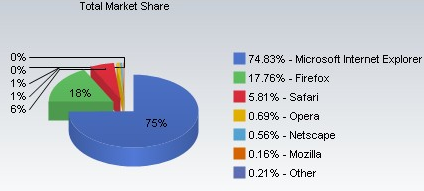
\includegraphics{browsers.png}
  \caption{
  Udział procentowy w rynku przeglądarek internetowych.\newline
  \emph{Źródło: http://marketshare.hitslink.com/report.aspx?qprid=0}
  \label{fig:przegladarki}
  }
\end{figure}

Niestety silniki nie są ze sobą ze sobą kompatybilne, każdy trochę inaczej interpretuje HTML, CSS, JavaScript, nie wszystkie mają wbudowane najnowsze technologie w tym samym stopniu. Największe trudności sprawia programistom przeglądarka Internet Explorer w wersji 6, która zajmuje największą część rynku i zarazem jest najbardziej przestarzałą (2001 r.). Ta wersja jest niezgodna ze standardami zatwierdzonymi przez W3C i posiada wiele błędów, często nazywana jest ,,zmorą programistów''. Niestety przeglądarka IE 6 wygrała pierwszą ,,wojnę przeglądarek''\footnote{Zobacz \url{http://en.wikipedia.org/wiki/Browser_wars}} i niemalże zmonopolizowała rynek. Następna wersja Internet Explorera (wersja 7) pojawiła się dopiero pod koniec 2006 roku. Zanim wersja 6 zniknie z rynku minie jeszcze kilka lat, w czasie których rozwój aplikacji po stronie klienta będzie ograniczony możliwościami tej przeglądarki.

\chapter[Rozwiązania koncepcyjne]{Koncepcje spotykane w aplikacjach internetowych}
\label{cha:koncepcje}

\section{Model-view-controller}
\label{sec:mvc}
MVC (ang. Model-view-controller, model-widok-kontroler) to wzorzec projektowy stosowany szeroko w informatyce, niemniej największą popularność zyskał w Internecie. Odpowiednie użycie wzorca oddziela logikę biznesową od warstwy prezentacji, co w efekcie przekłada się na możliwość zmiany wyglądu aplikacji bez wpływu na logikę biznesową i odwrotnie. W MVC Model reprezentuje informacje o aplikacji i założeniach biznesowych użytych w celu obróbki danych. Widok, odpowiada za elementy UI (ang. User Interface, interfejs użytkownika) takie jak tekst, listy, pola wyboru etc. Kontroler spaja wszystko w całość pośrednicząc między Modelem a Widokiem i zajmując się sterowaniem.

\subsection{Krótka Historia}
\label{subsec:mvc-historia}
Wzorzec został po raz pierwszy opisany w 1979~r.\footnote{Zobacz \url{http://heim.ifi.uio.no/~trygver/themes/mvc/mvc-index.html}} przez Trygve Reenskaug wtedy pracującegp w XEROX~PARC nad językiem Smalltalk\footnote{Zobacz \url{http://www.smalltalk.org/}} Oryginalna implementacja została dokładnie opisana w dokumencie \emph{Applications Programming in Smalltalk-80: How to use Model-View-Controller.}\footnote{Zobacz \url{http://st-www.cs.uiuc.edu/users/smarch/st-docs/mvc.html}}.

Po pewnym czasie, powstało wiele wariacji na temat koncepcji, dość wspomnieć o wzorcu Model-view-presenter, który powstał początkiem lat 90 i został zaprojektowany jako następca MVC. Nie zmienia to faktu, że MVC trzyma się mocno i wciąż znajduje szerokie zastosowanie.

\subsection{Opis wzorca}
\label{subsec:mvc-opis}
Dość powszechnie stosowaniem rozwiązaniem jest dzielenie aplikacji na warstwę prezentacji i warstwę logiczną. MVC idzie o krok dalej, dzieląc warstwę prezentacji na Widok i Kontroler. Kładzie on też większy nacisk na architekturę aplikacji niż typowy wzorzec projektowy. Trzy jego główne elementy to:
\begin{itemize}
  \item \emph{Model} - Specyficzna dla każdego projektu reprezentacja informacji, na których działa aplikacja. Jest to DSL (ang. Domain Specific Language, zob.~r.~\ref{sec:dsl} str.~\pageref{sec:dsl}), który opisuje i operuje na surowych danych (np. obliczenie czy dzisiaj użytkownik obchodzi urodziny, kosztu wszystkich towarów w koszyku etc.). Wiele aplikacji wykorzystuje ściśle określony mechanizm przechowywania danych (w przypadku aplikacji internetowych, prawie zawsze jest to baza danych). MVC sam w sobie, nie określa metody przechowywania danych, ponieważ założenie jest takie, że danymi zajmuje się model.
  \item \emph{Widok} - Przedstawia dane z modelu w postaci czytelnej dla użytkownika. MVC nie definiuje ścisłej relacji ilościowej pomiędzy Modelami a Widokami, co oznacza, że jeden Model może obsługiwać wiele widoków jak i jeden Widok może otrzymywać dane od wielu Modeli.
  \item \emph{Kontroler} - Odpowiada za proces interakcji między aplikacją użytkownikiem. Pobiera ,,zapytania'' od użytkownika i przekazuje je Modelowi. Następnie zwraca użytkownikowi nowy widok z nowymi informacjami. Może również dokonywać zmian w samym Modelu.
\end{itemize}

\subsection{Zastosowanie w aplikacjach internetowych}
\label{subsec:mvc-web}
MVC często znajduje zastosowanie w aplikacjach internetowych, gdzie widokiem jest aktualnie wyświetlana strona WWW, a kontroler to kod, który pobiera dane dynamiczne i wypełnia nimi HTML. Model z kolei reprezentuje dane (zazwyczaj przechowywane w bazie danych lub plikach XML) oraz reguły biznesowe, które zamieniają te dane na informację przedstawianą potem użytkownikowi.

Mimo, że MVC jest dostarczany w wielu frameworkach, z których każdy ma odmienny pomysł na jego implementację, generalna zasada jest taka sama:
\begin{enumerate}
  \item Użytkownik wykonuje jakąś akcję w UI (np. wciska guzik).
  \item Kontroler obsługuje nadchodzące wywołanie, często wykorzystując jakąs metodę lub odwołanie.
  \item Kontroler informuje model o akcji użytkownika, czasami również modyfikuje jego stan (np. Kontroler uaktualnia zawartość koszyka).
  \item Widok wykorzystuje model (pośrednio) do wygenerowania odpowiedniego interfejsu użytkownika (np. wyświetla tabelkę z zakupami). Widok pobiera dane z modelu, ale sam model nic nie wie o Widoku.
  \item UI oczekuje na kolejną akcję, co rozpoczyna cały cykl od początku.
\end{enumerate}

Rozdzielając Modele od Widoków, MVC znacznie zmniejsza skomplikowanie architektury programu i zwiększa przejrzystość i elastyczność.

\section{Object-relational mapping}
\label{sec:orm}
Mapowanie obiektowo-relacyjne (z ang. Object-relational mapping) jest techniką programistyczną stosowaną do konwersji danych przy niekompatybilnych ze sobą relacyjnych baz danych i obiektowo zorientowanych językach programowania. W efekcie otrzymywany jest ,,wirtualny obiekt bazy danych'', który może być następnie użyty na poziomie kodu zadanego języka programowania. Istnieją zarówno darmowe jak i komercyjne rozwiązanie ORM, niemniej sporo programistów wciąż tworzy swoje rozwiązania.

\subsection{Opis problemu}
\label{subsec:orm-problem}
Zarządzanie danymi w programowaniu obiektowym zazwyczaj jest rozwiązane jako manipulowanie różnego rodzaju obiektami, które prawie nigdy nie są wielkościami skalarnymi. Dla przykładu, dany jest obiekt reprezentujący osobę w książce teleadresowej. Osoba taka, może mieć kilka telefonów i kilka adresów (zameldowania, zamieszkania etc.). Obiekt reprezentujący taką osobę miałby kilka ,,slotów'', które zawierałyby kolejno, dane osobowe, listę telefonów i listę adresów. Oczywiście, lista telefonów może z kolei zawierać obiekty numerów telefonów (z osobnym slotem, na operatora, numer kierunkowy etc.), lista adresów obiekt adresu itd. Dodatkowo, wszystkie te obiekty miałyby swoje własne metody, np. do zwracania telefonu domowego, preferowanego adresu itd.

Z drugiej strony, bazy danych mogą przechowywać tylko dane skalarne zorganizowane w tabelach.

Programista musi więc albo zorganizować podobne wartości obiektów jako dane dla tabeli, albo całkowicie uprościć strukturę kodu, do poziomu wartości skalarnych aby potem bezproblemowo umieszczać je w bazie. Podejście ORM wykorzystuje pierwsze rozwiązanie.

Cały problem polega na takiej organizacji tych obiektów, aby potem dało się je łatwo zapisać do bazy, jednocześnie nie tracąc samej struktury obiektu (w celu późniejszego odczytu). Obiekty takie muszą być więc przenaszalne między kodem a bazą danych.

\subsection{Implementacje}
\label{subsec:orm-implementacje}
Najpowszechniej stosowanym rozwiązaniem jest relacyjna baza danych, która poprzedziła narodziny ORM w 1990 r. Relacyjne bazy danych, wykorzystują serie tabel do organizacji danych. Dane w różnych tabelach są ze sobą powiązane przy pomocy kluczy założonych na całe kolumny, a nie na poszczególne wartości. Może się okazać, że dane przechowywane w jednym obiekcie muszą być rozłożone na kilka tabel.

ORM powinien systemacznie przewidywać jakie tabele będą potrzebne do zapisania określonych obiektów i generować odpowiednie zapytania SQL. Różnice między sposobem prezentacji danych w modelu obiektowo zorientowanym (w takich językach jak Java, C\# czy Ruby) a sposobem ich przechowywania w relacyjnej bazie danych (takiej jak Oracle czy PostgreSQL), pociągają za sobą następujące problemy:
\begin{itemize}
  \item Wydajność,
  \item Skalowalność,
  \item Zarządzanie operacjami typu CRUD (patrz rozdz.~\ref{sec:crud}, str.~\pageref{sec:crud}) dla bardziej skomplikowanych relacji,
  \item Uproszczenie i spójność kodu konieczna przy szybkim tworzeniu aplikacji,
  \item Zarządzanie i elastyczność kodu.
\end{itemize}

Prawdziwą wartością ORM jest przedewszystkim oszczędność czasu i uproszczenie kodu (wszystkie skomplikowane operacje bazodanowe ORM załatwia za programistę). Dodatkowo ORM zwiększa wydajność i skalowalność oraz minimalizuje problemy niekompatybilności architektur (dobry ORM obsługuje większość obecnie stosowanych systemów baz danych).

Powstało sporo aplikacji ORM, które dostarczając zestaw klas i bibliotek autmatyzują proces mapowania i odciążają programistę. Po podaniu im listy tabel w bazie, same wygenerują odpowiednie obiekty i relacje między nimi. Wracając do poprzedniego przykładu -- pytając taki obiekt o numer telefonu, w tle nastąpi utworzenie zapytania SQL, wysłanie go do bazy, przetworzenie wyniku a następnie konwersja do postaci zgodnej z obiektem.

Z punktu widzenia programisty, nie powinno go zajmować jak to wszystko się odbywa -- powinien tylko wiedzieć, że zapisanie danej do obiektu, skutkuje zapisaniem jej w bazie.

W praktyce nie jest to takie proste. Nie jest możliwe stuprocentowe zmapowanie wszystkich możliwych kombinacji zapytań. Wszystkie ORM mają margines błędu, który użytkownik może zniwelować tylko poprzez bezpośrednie wysłanie zapytania SQL do bazy. Dodatkowo, cały proces mapowania i unifikacji zapytań pociąga za sobą spadek wydajności (zapytania SQL z poziomu ORM są tworzone z myślą o jak największej elastyczności i uniwersalności, więc niekoniecznie muszą być najszybsze dla konkretnego przypadku).

\subsection{Zastosowanie w aplikacjach internetowych}
\label{subsec:orm-web}
Koncepcja ORM jest wykorzystywana we wszystkich nowoczesnych frameworkach webowych, ponieważ ściąga z programisty konieczność dbania o spójność danych w bazie, utrzymywania i rozłączania połączeń etc. Nie bez znaczenia jest też wsparcie dla różnych architektur bazodanowych. Często dzieje się tak, że po przeniesieniu aplikacji na nowy serwer okazuje się, że baza danych zmieniła się. Wtedy wystarczy tylko jedna zmiana w pliku konfiguracyjnym, a całość powinna zadziałać automatycznie.

Drugą, znaczącą zaletą jest to, że ORM wymusza spójność kodu (przynajmniej w kwestii obsługi bazy danych) -- oznacza to, że przy projektach pisanych przez wielu programistów, jest znacznie mniej niespójności i nieścisłości -- wszyscy trzymają się jednej konwencji.

\section{Representational State Transfer}
\label{sec:rest}
REST (ang. REpresentional State Transfer, reprezentacja stanu transferu) jest to styl w architekturze programowania przeznaczony dla multimedialnych systemów rozproszonych takich jak World Wide Web. Określenia ,,Representional state transfer'' i ,,REST'' zostały pierwszy raz zaprezentowane w 2000 roku na rozprawie doktorskiej, którą przeprowadzał Roy Fielding\footnote{Zobacz http://www.ics.uci.edu/~fielding/pubs/dissertation/rest\_arch\_style.htm} -- jeden z głównych autorów specyfikacji protokołu HTTP. Zwroty te, szybko rozpowszechniły się wśród sieciowej społeczności.

REST ściśle odnosi się do założeń sieciowych, które określają jak zasoby są definiowane i adresowane. Określenie to, jest też często używane w luźnym sensie, do opisania jakiegokolwiek prostego interfejsu, który przesyła informacje określone w danej domenie (patrz rozdz.~\ref{sec:dsl}, str.~\pageref{sec:dsl}) poprzez protokół HTTP wraz z dodatkową warstwą wiadomości, taką jak SOAP czy też kontrolą sesji wykorzystującą ,,ciasteczka''. Oba te określenia mogą budzić konflikt, jak i się uzupełniać. Jest możliwe zaprojektowanie dużej, skomplikowanej aplikacji w metodologii REST, jednocześnie nie używając HTTP i nie łączac jej z WWW. Jednakże, jest także możliwe zbudowanie prostej aplikacji XML+HTTP, która zupełnie nie spełnia założeń REST. Te różnice w używaniu terminu ,,REST'', często prowadzą do pewnego zakłopotania w technicznych dyskusjach.

Systemy, które spełniają założenia REST, często bywają określane jako ,,RESTful''.

\subsection{Założenia}
\label{sub:rest-zalozenia}
Najważniejszym założeniem w REST jest istnienie zasobów (źródeł określonej informacji), z których każdy może być zaadresowany używając globalnego odnośnika URI (ang. Uniform Resource Identifier, jednoznaczny identyfikator zasobu). Aby modyfikować te zasoby, komponenty sieci (klienci i serwery) komunikują się między sobą przez zestandarazywany interfejs (np. HTTP) i wymieniają między sobą reprezentacje tych zasobów (dokumenty zawierające określone informacje). Dla przykładu zasób ,,okrąg'' może przyjmować i zwracać reprezentację w postaci współrzędnych środka i promienia, skonwertowaną do formatu SVG, ale może też to być plik tekstowy zawierający trzy współrzędne po średniku, które lężąc na tym okręgu definiują go jednoznacznie.

Orędownicy REST utrzymują, że skalowalność i rozwój sieci są bezpośrednią przyczyną kilku kluczowych założeń:
\begin{itemize}
  \item Stany i funkcjonalności aplikacji są podzielone między zasoby,
  \item Każdy zasób jest unikalnie adresowalny używając uniwersalnej składni wykorzystywanej do tworzenia odnośników,
  \item Wszystkie zasoby dzielą jednolity interfejs do transportu stanów pomiędzy klientem a zasobem, zawierający:
  \begin{itemize}
    \item Ograniczony zestaw dobrze opisanych rozkazów,
    \item Ograniczony zestaw typów danych, może jednak być wysłany w ramach ,,kodu na żądanie''.
  \end{itemize}
  \item Protokół, którego cechami są:
  \begin{itemize}
    \item Klient-serwer,
    \item Bezstanowość,
    \item Cacheowalność,
    \item Warstwowość.
  \end{itemize}
\end{itemize}

\subsection{Zastosowanie w aplikacjach internetowych}
\label{rest:web}

World Wide Web jest kluczowym przykładem projektu typu ,,RESTful''. Większość założeń WWW, pokrywa się z założeniami REST. Sieć opiera się na protokole HTTP, prezentacji treści w postaci dokumentów HTML oraz różnych innych technologii internetowych, jak np. DNS (Domain Name System, system nazw domenowych).

HTML może zawierać JavaScript i applety aby wspierać kod na żądanie, oraz posiada wbudowaną obsługę hyperlinków.

HTTP jest jednolitym interfejsem dostępu do zasobów, który zawiera URI, metody, kody stanu, nagłówki i zawartość opisaną MIME type (ang. Multipurpose Internet Mail Extensions, rozszerzenia poczty internetowej stosowane do różnych celów).

Najważniejszymi metodami HTTP są POST, GET, PUT i DELETE (patrz rozdz.~\ref{sec:http}, str.~\pageref{sec:http}). Są one często porównywane do CREATE, READ, UPDATE i DELETE (CRUD, patrz rozdz.~\ref{sec:crud}, str.~\pageref{sec:crud}), które to pojęcia mają zastosowanie w bazach danych.

\begin{table}[h]
  \centering
    \begin{tabular}{|l|l|}\hline
    HTTP   & CRUD \\\hline
    POST   & Create, Update, Delete \\
    GET    & Read \\
    PUT    & Create, Update \\
    DELETE & Delete \\\hline
    \end{tabular}
  \caption{Porównanie zapytań HTTP z koncepcją CRUD\label{rest:crud}}
\end{table}

HTTP spełnia jedno z założen REST -- jest bezstanowy. Każda wiadomość zawiera wszystkie informacje niezbędne do identyfikacji zapytania. W efekcie czego, ani klient ani serwer nie muszą pamiętać żadnych stanów informacyjnych pomiędzy wiadomościami. Każdy stan w którym jest serwer, może być zamodelowany jako zasób.

Ta bezstanowość może być naruszona w HTTP, kiedy używamy ciasteczek do podtrzymywania sesji. Używanie ciasteczek często wiąże się z naruszeniami polityki prywatności i problemami bezpieczeństwa. Dodatkowo, pojawia się wiele nieścisłości i błędów jeśli do problemów z ciasteczkami dołożymy jeszcze obecność przycisku ,,wstecz'' w przeglądarce.

Nie bez znaczenia jest też fakt, że hipertekst HTML tak naprawdę pozwala tylko na użycie zapytań typu ,,GET''. Dodatkowo jest jeszcze dostępny ,,POST'' dzięki formularzom. Pozostałe metody HTTP nie są wspierane ani przez HTML~4.01 ani XHTML~1.0.\footnote{Więcej informacji na http://www.w3.org/TR/2007/REC-wsdl20-adjuncts-20070626/\#\_http\_binding\_default\_rule\_method}

\section{Domain Specific Language}
\label{sec:dsl}
DSL (z ang. Domain Specific Language, język określonego przeznaczenia) to język zaprojektowany w ściśle określonym celu. W przeciwieństwie do języków ogólnego przeznaczenia takich jak Java czy C, których zadaniem jest uniwersalność i możliwość zastosowania w jak największej liczbie przypadków, DSLe są projektowane tylko w jednym, ściśle określonym celu. Przykładem DSLa jest np. język SQL - zaprojektowany tylko i wyłącznie do obsługi baz danych. Termin DSL nie jest terminem nowym, jednak dopiero ostatnio zyskał sobie sporą popularność. Powodem tego jest znaczny wzrost mocy obliczeniowej komputerów oraz elastyczność nowych języków generalnego przeznaczenia, która umożliwia pisanie własnych DSL.

\subsection{Przykłady zastosowań}
\label{sub:zastosowania}

Można wykazać conajmniej kilka przykładów zastosowań dla DSL:
\begin{enumerate}
  \item wykorzystywanie samodzielnych aplikacji wywoływanych przez bezpośrednią akcję użytkownika (najczęściej z poziomu linii poleceń lub pliku Makefile), np. zestaw narzędzi GraphViz
  \item DSL, które są zaimplementowane przy użyciu systemów makr, a następnie są konwertowane lub rozszerzane do trybu zgodności z nadrzędnym językiem programowania ogólnego przeznacznia, podczas fazy kompilacji lub interpretowania
  \item DSL w całości napisane w języku programowania ogólnego przeznaczenia (takim jak C lub Perl), mające na celu wykonywanie określonych operacji i zwracanie danych, które język nadrzędny jest w stanie zrozumieć i przetworzyć. Generalnie, taki DSL można rozumieć jako język programowania szczególnego przeznaczenia napisany w języku programowania ogólnego przeznaczenia.
  \item DSL, które są częścią aplikacji w której pracują -- dobrym przykładem są tu różnego rodzaju systemy makr w arkuszach kalkulacyjnych, wykorzystywane do uruchamiania specyficznych funkcji napisanych przez użytkownika, lub tworzone dynamicznie przez samą aplikację.
\end{enumerate}

Wiele DSL może być używane w kilku powyższych przypadkach naraz.

\subsection{Zastosowanie w aplikacjach internetowych}
\label{dsl:web}
W aplikacjach internetowych DSL znalazły szerokie zastosowanie przy zadaniach często powtarzających się, takich jak na przykład tworzenie modeli, testy czy obsługa baz danych. Nie można również zapomnieć o najważniejszym z DSL z punktu widzenia WWW -- o SQL. Bez niego istnienie większości serwisów internetowych byłoby praktycznie niemożliwe. DSL świetnie też się sprawdzają w całej otoczce okołoaplikacyjnej. Używając ich, można zautomatyzować procesy takie jak:
\begin{itemize}
  \item Wysyłanie aplikacji na serwer
  \item Synchronizacja z systemem kontroli wersji np. SVN (z ang. SubVersioN)
  \item Testowanie aplikacji oraz jej poszczególnych komponentów
  \item Wiele różnych akcji związanych z przejściem z trybu developerskiego na produkcyjny, jak np.:
  \begin{itemize}
    \item Kompresja i obfuskacja (zaciemnienie) plików JavaScript
    \item Kompresja CSS
    \item Usuwanie informacji o gammie z plików PNG (ang. Portable Network Graphics, przenośna grafika sieciowa)
    \item Zmiany nazw plików aby zostały ponownie pobrane (dotyczy to w szczególności serwisów, gdzie wymuszany jest nieskończony czas cacheowania plików przez przeglądarkę)
    \item Czyszczenie różnych pozostałości developerskich (stare, skompilowane pliki szablonów, logi, etc.)
  \end{itemize}
\end{itemize}

\section{Create, Read, Update and Delete}
\label{sec:crud}
CRUD (Create, read, update and delete -- utwórz, odczytaj, popraw i skasuj) są to cztery podstawowe funkcje dotyczące operacji na danych, najważniejszej czynności w całej informatyce. Czasami w skrócie tym, zamiast ,,read'' używa się ,,restore'' a zamiast ,,delete'' -- ,,destroy''. Często jest stosowany przy opisywaniu operacji na bazach danych lub przy opisie interfejsów.

\subsection{CRUD w relacyjnych bazach danych}
\label{sub:crud-db}
Akronim CRUD jest często odnoszony do relacyjnych baz danych, ponieważ te cztery operacje determinują zupełność takiej bazy danych. Każda litera akronimu, może zostać przedstawiona jako odpowiednia funkcja SQL:
\begin{table}[h]
  \centering
    \begin{tabular}{|l|l|} \hline
    Operacja         & SQL \\\hline
    Create           & INSERT \\
    Read (Retrieve)  & SELECT \\
    Update           & UPDATE \\
    Delete (Destroy) & DELETE \\\hline
    \end{tabular}
    \caption{Mapa akronimu CRUD na zapytania SQL\label{crud:sql}}
\end{table}
Pomimo iż CRUD głównie odnosi się do relacyjnych baz danych, często jest też stosowany w odniesieniu do obiektorych baz danych, XMLowych baz danych, plików tekstowych, nośników informacji etc.

\subsection{Zastosowanie w aplikacjach internetowych}
\label{crud:web}
W aplikacjach internetowych, CRUD odnosi się do samego interfejsu. Dla przykładu, jeśli tworzona jest książka teleadresowa, podstawową jednostką danych jest informacja o kontakcie. Jako niezbędne minimum, aplikacja musi:

\begin{itemize}
  \item Utworzyć lub dodać nowy kontakt (Create)
  \item Wyświetlić istniejące wpisy (Read)
  \item Zmieniać niektóre informacje (Update)
  \item Usuwać niepotrzebne kontakty (Delete)
\end{itemize}

Bez którejkolwiek z powyższych operacji, aplikacja nie może być uznana za kompletną. Zasada ta, też jest podwaliną każdego dobrego frameworka, gdyż zautomatyzowanie jej, znacznie skraca czas tworzenia programu.

\section{Don't Repeat Yourself}
\label{sec:dry}
DRY (z ang. Don't Repeat Yourself, nie powtarzaj się) jest filozofią, której celem nadrzędnym jest zredukowanie duplikatów. Występuje głównie w informatyce. DRY zakłada, że ta sama informacja nie powinna być powielana w ramach jednego projektu, gdyż taka duplikacja znacznie utrodnia zmiany, zmniejsza czytelność i prowadzi do niespójności. Don't Repeat Yourself jest głównym przykazaniem książki \emph{The Pragmatic Programmer}\footnote{TODO: BIBLIOGRAFIA}, której autorami są Andy Hunt i Dave Thomas. W publikacji tej, zalecają, aby używać jej w jak najszerszym zakresie, włączając ,,schematy baz danych, plany testów, budowany system a nawet dokumentacje''\footnote{Wywiad Billa Vennersa z Dave Thomasem \emph{Orthogonality and the DRY Principle}, zob.~\url{http://www.artima.com/intv/dry.html}}. Kiedy reguła DRY zostanie pomyślnie wdrożona w system, jakakolwiek zmiana jakiegoś elementu w kodzie, nie wpłynie w żaden sposób na elementy nie będące z nim logicznie połączone. Dodatkowo, wszystkie elementy logicznie połączone ze zmienionym, zmienią się w sposób przewidywalny i wciąż będą ze sobą zsynchronizowane.

\subsection{Kiedy DRY może się nie sprawdzić}
\label{sub:dry-not}
Reguła DRY nie zawsze się sprawdza i w niektórych przypadkach, lepiej z niej zrezygnować:
\begin{itemize}
  \item W małych projektach, albo prostych skryptach, wysiłek jaki trzebaby było włożyć aby trzymać się reguły DRY, byłby znacznie większy niż proste napisanie dwóch kopii tej samej danej w różnych miejscach,
  \item Wymuszanie DRY w projektach, w których najważniejszą rolę w tworzeniu treści pełni społeczność (np. wikipedia), mogłoby znacznie ostudzić zapał ludzi do tworzenia nowych wpisów,
  \item Zarządzanie projektami i kontrolą wersji pozwala (a nawet) zaleca tworzenie kilku kopii, bez wykorzystywania DRY. Dla przykładu, bardzo dobrym nawykiem jest tworzenie trzech środowisk dla jednej aplikacji -- produkcyjnego, testowego i deweloperskiego. Dzięki temu mamy pewność, że rozwojowy albo testowy kod, nie będzie miał wpływu na stabilne wersje produkcyjne,
  \item Dokumentacja dla użytkowników końcowych (od komentarzy w kodzie, do drukowanych instrukcji) zawiera typowe informacje opisujące pewnie funkcjonalności kodu, przeznaczone dla ludzi, którzy nie potrzebują lub nie mają czasu analizować całego listingu programu. Niestety DRY zakłada, że jeśli taka dokumentacja nie stanowi jakiejś wartości dla samego kodu (a nie dla użytkowników), to powinna być generowana a nie pisana,
  \item Generatory kodu źródłowego - niepowtarzalność będzie skuteczna dla generatora samego w sobie, ale nie musi już być konieczna dla samego wygenerowanego źródła, które jest używane automatycznie i nikt nie będzie do niego zaglądał ani go zmieniał.
\end{itemize}

\subsection{Zastosowanie w aplikacjach internetowych}
\label{dry:web}
Reguła DRY świetnie sprawdza się we wszystkich projektach programistycznych, ale największe uznanie znalazła właśnie wśród programistów aplikacji internetowych. Specyfika internetu jest inna niż desktopu -- wszystkie zmiany zachodzą dużo szybciej. Czas życia przeciętnego projektu internetowego to kilka lat i w tym czasie musi on podlegać ciągłemu rozwojowi i przemianom. Gdyby nie DRY, zmiany zachodziły by dużo wolniej, byłyby dużo trudniejsze do przeprowadzenia i pochłaniałyby więcej środków. Filozofia DRY (oczywiście w pełni respektowana) wymusza na programistach WWW porządek w kodzie dzięki czemu taka aplikacja jest w stanie szybko przystosować się do zmiennych warunków rynkowych.

\section{Convention over Configuration}
\label{sec:coc}
Convention over Configuration (konwencje ponad konfiguracje) jest jedną metodologii projektowania oprogramowania, która dąży do osiągnięcia minimalizacji ilości decyzji jakie muszą podjąć deweloperzy, zyskując dzięki temu prostotę bez utraty elastyczności.

Sformułowanie samo w sobie oznacza, ze programista musi rozpatrywać tylko niekonwencjonalne aspekty aplikacji. Dla przykładu, jeśli dana jest klasa \emph{Sprzedaż} obsługująca model, to przypisana jej tabela jest domyślnie również nazwana ,,sprzedaż''. Jeżeli teraz nie zostanie naruszona konwencja (czyli np. tabela nie zostanie nazwana ,,sprzedaż\_produktów''), to programista nie musi nigdzie określać nazwy tabeli i potem odwoływać się do niej w innych miejscach.

Im więcej dobrych konwencji w kodzie, tym na wyższym poziomie abstrakcji może się skupić programista, co oznacza, że mocniej zajmuje się aspektami logicznymi zagadnienia, a nie technicznymi.

\subsection{Geneza}
\label{sub:geneza}
Tradycyjnie, frameworki potrzebowały ogromnej ilości różnych plików konfiguracyjnych, z których każdy opisywał inne ustawienie. Pliki te zawierały specyficzne informacje dla każdego projektu, zawierające wszystko -- od mapowania URL, poprzez klasy aż po konfiguracje tabel w bazie danych. Przy większym skomplikowaniu aplikacji rozmiar i liczba tych plików powiększała się.

Dobrym przykładem jest tutaj ORM (zob. rozdz.~\ref{sec:orm}, str.~\pageref{sec:orm}) Hibernate. Mapuje on tabele w bazach danych na świat obiektowy, wykorzystując w tym celu pliki XML. Większość informacji jest konwertowanych w myśl z góry ustalonych zasad. Nazwy klas, są mapowane na identycznie nazwane tabele w bazie danych, a ich wartości -- na kolumny. Jest to konwencja ustalona przez deweloperów Hibernate i narzucona użytkownikom, tj. programistom, którzy używają tego frameworka. Oczywiście nic na siłę i jeśli któryś programista potrzebuje, aby nazwy się różniły, zawsze może sobie ustalić wszystkie wyjątki w odpowiednim pliku konfiguracyjnym.

\subsection{Zastosowanie w aplikacjach internetowych}
\label{coc:web}
Convention over Configuration, jest koncepcją stosunkowo młodą w światku internetowym, ale z miejsca zdobyła sobie rzesze zwolenników. Wynika to przedewszystkim z tego, że upraszcza wiele aspektów i sprawia, że z każdym nowym projektem deweloperzy nie muszą wciąż skupiać się na tych samych problemach. Poza tym, przy większych aplikacjach nad którymi pracują dziesiątki programistów, konwencje sprawiają, że każdy pisze w ten sam sposób i nie ma problemów w rodzaju -- ,,Co ta metoda robi?''. Dodatkowo złamanie konwencji wiąże się ze sporą nadprodukcją kodu, co niejako ,,samo z siebie'' wymusza w programistach dyscyplinę.

\chapter{Aplikacja}
\label{cha:app}
Serwis WWW zadany w temacie pracy był od początku z góry ustalony. Jest to strona Katedry Elektroniki i Telekomunikacji\footnote{Zobacz. http://www.eit.agh.edu.pl/}. Motywem przewodnim takiego wyboru była przestarzałość serwisu i niespójność kodu. Przez kilka lat od momentu stworzenia, aplikację rozwijało wiele różnych osób, skutkiem czego kod zatracił swoją początkową ,,myśl przewodnią'' oraz znacznie stracił na czytelności. Dlaczego więc nie zdecydowane się na przepisanie serwisu od nowa, również w PHP? Głównym powodem była ,,samoopisywalność'' kodu stworzonego w Ruby~on~Rails. Dzięki filozofii DRY (zob. rozdz.~\ref{sec:dry}, str.~\pageref{sec:dry}) oraz Convention over Configuration (zob. rozdz.~\ref{sec:coc}, str.~\pageref{sec:coc}) każdy kawałek kodu ma ściśle określone miejsce w aplikacji. Dodatkowo sama struktura plików projektu Railsowego jest klarowna i przejrzysta. Zawsze w tym samym miejscu przechowywane są modele, widoki, biblioteki, kontrolery itd. Dzięki temu, kiedy autor niniejszej pracy przekaże serwis w ręce nowego programisty, już na starcie będzie on doskonale wiedział, gdzie czego szukać. Dodatkowo czytelność kodu Ruby i łatwość tworzenia DSL (zob. rozdz.~\ref{sec:dsl}, str.~\pageref{sec:dsl}) sprawia, że taki kod od razu przekazuje ,,co autor miał na myśli''. I stąd właśnie bierze się jego samoopisywalność.

\section{Opis funkcjonalny aplikacji}
\label{sec:funkcjonalny}
Głównym założeniem serwisu Katedry Elektroniki i Telekomunikacji (zwanego dalej EiT) jest stworzenie portalu zawierającego wszelkie niezbędne studentowi informacje. Na funkcjonalności te składają się przedewszystkim:
\begin{itemize}
  \item System aktualności i najświeższych informacji dla studentów,
  \item Wszelkie informacje pochodzące z dziekanatu, m.in. informacje o:
  \begin{itemize}
    \item planach zajęć,
    \item praktykach,
    \item przedmiotach obieralnych,
    \item zajęciach w języku angielskim,
    \item międzynarodowym programie edukacyjnym,
    \item wydarzeniach obowiązkowych w kalendarzu studenta (ferie, sesje etc.).
  \end{itemize}
  \item System zarządzania materiałami i ocenami,
  \item Informacje o prowadzących,
  \item Wszelkie dane dotyczące studiów podyplomowych.
\end{itemize}
Dodatkowo należało jeszcze zatroszczyć się o całą warstwę administracyjną. Grupa ludzi opiekujących się stroną (zwanych dalej Administratorami) powinna mieć specjalne uprawnienia, do dodawania informacji, usuwania niepotrzebnych treści, zarządzania studentami (z poziomu systemu) itd. Dodatkowo, wszyscy prowadzący powinni mieć możliwość dodawania aktualności i materiałów. 

Wymienione powyżej funkcjonalności autor tej pracy wspólnie z prowadzącym uznał za najważniejsze i umieścił je w serwisie. Stara strona EiT miała jeszcze dodatkowo forum i katalog linków. Autor wspólnie z opiekunem, uznali je jednak za zbyteczne. W obu przypadkach głównym powodem było znikome zainteresowanie studentów. Katalog linków nie sprawdził się, ponieważ tak naprawdę wszystkie informacje były dostępne z poziomu serwisu i nie były potrzebne żadne referencje do innych witryn. Forum z kolei (zwane Hydeparkiem) przestało pełnić swoją pierwotną funkcję. W dzisiejszych czasach istnieją setki serwisów pozwalające założyć darmowe forum jednym kliknięciem myszki. I właśnie na takie biuletyny przenieśli się studencji, tworząc fora swoich roków bądź grup dziekanatowych. Nie bez znaczenia jest też fakt, że do Hydeparku dostęp mieli prowadzący co z miejsca ucinało niektóre rodzaje konwersacji.

Kolejną niesłychanie istotną cechą serwisu jest jego bezpieczeństwo. W przypadku serwisu EiT sprawa jest o tyle poważna, że jest to aplikacja przeznaczona dla ludzi technicznych, którzy doskonale orientują w świecie nowoczesnych technologii. Najmniejsze niedopatrzenie może się zakończyć kompromitacją serwisu. Autor niniejszej pracy od wielu lat zajmuje się tematyką szeroko pojętego bezpieczeństwa. I to zarówno od strony aplikacyjnej (pisanie bezpiecznego kodu) jak i serwerowej (zabezpieczanie maszyn przed intruzami). W związku z tym, od początku każdy element witryny był szczegółowo rozważany pod tym kątem. Nie bez znaczenia jest też fakt, że Ruby~on~Rails przychodzi z wieloma rozwiązaniami ochronnymi w standardzie. Dla przykładu jeśli nastąpi jakiś błąd w działającej aplikacji, to w odróżnieniu od PHP nie pojawi się komunikat dokładnie informujący, która linijka w którym skrypcie go wywołała. Zamiast tego, wyświetli się informacja dla użytkownika, że ,,coś poszło nie tak'' a sam błąd zostanie zapisany do logów administratora. Dzięki temu, potencjalny atakujący nie otrzymuje żadnej informacji o serwisie, poza tym, że działając tak i tak można uszkodzić aplikację -- co jakąś wartościową informacją samo w sobie nie jest.

Należy też pamiętać o interfejsie użytkownika. Sama szata graficzna pozostała niezmieniona, natomiast musiał zmienić się jej kod. Wynika to z zupełnie nowej filozofii tworzenia widoków. Poza tym, stary kod HTML nie był w ogóle semantyczny, co znacznie utrudniało pracę robotom wyszukiwarek i skutkowało niższymi pozycjami w rankingach. Cały HTML został przepisany na nowo (już jako XHTML) i stworzone zostały nowe arkusze stylów. Zmieniła się też organizacja menu -- kliknięcie w menu nie odświeża strony tylko od razu rozwija listę podmenu. Zmniejsza to znacznie ilość zapytań (wcześniej student musiał otworzyć nową stronę, tylko po to, żeby zobaczyć rozwinięte menu i przejść do kolejnej strony) oraz skraca czas interakcji użytkownika ze stroną. A wszystko to, dzięki odrobinie JavaScriptu.

Ostatnią sprawą jest wydajność. Jak już nadmienione zostało wcześniej -- Ruby nie jest zbyt szybkim językiem. Dlatego wszelkie działania mające na celu optymalizację kodu są wysoce wymagane. Bardzo istotne jest zwracanie uwagi na takie detale, jak wyciąganie deklaracji zmiennych poza pętle, optymalizacje warunków (ważna jest tu znajomość praw deMorgana), przypisywanie obiektów do zmiennych etc. Zastosowany też został dużo wydajniejszy serwer WWW aniżeli dostarczany w standarcie WebRick --- Mongrel\footnote{Zobacz \url{http://mongrel.rubyforge.org/}}

\section{Przygotowanie środowiska pracy}
\label{sec:srodowisko}
Po przygotowaniu założeń należało wybrać środowisko pracy.

\subsection{Ruby i pochodne}
\label{sub:ruby-etc}
Ruby jest językiem międzyplatformowym, co oznacza, że jego interpreter jest dostępny pod każdym liczącym się systemem operacyjnym. Niestety implementacja pod systemem Windows pozostawia wiele do życzenia. Bierze się to stąd, że Ruby został pierwotnie stworzony na systemach UNIXopodobnych a następnie przeportowany na platformę Windows. Przy takiej skali skomplikowania języka, brak optymalizacji pod konkretny system daje się odczuć. Różnice w czasach wykonania aplikacji potrafiły przekroczyć 100\%! Autor niniejszej pracy, korzysta z Linuksa a konkretniej z dystrybucji \emph{Slackware Linux}, natomiast do pracy z Ruby poleca jakąkolwiek dystrybucje UNIXopodobną (włączając to MAC~OS~X).

Slackware~12.0 ma interpreter Ruby w standardzie (przy maksymalnej instalacji). W razie jego braku, należy pobrać odpowiednią paczkę -- Ruby~1.8.6\footnote{Do pobrania m.in. na \url{http://linuxpackages.telecoms.bg/Slackware-11.0/ken/ruby-1.8.6-i486-1kjz.tgz}}. Do tego będą jeszcze protrzebne RubyGems~0.9.2\footnote{Do pobrania m.in. na \url{http://linuxpackages.telecoms.bg/Slackware-11.0/ken/rubygems-0.9.2-noarch-1kjz.tgz}}. Ponieważ Slackware nie obsługuje zależności, w razie problemów należy doinstalować brakujące biblioteki.

Po instalacji użytkownik otrzymuje w pełni funkcjonujący interpreter języka Ruby, w którym jednak brakuje jeszcze kilku bibliotek tego języka. Do ich instalacji należy posłużyć się narzędziem RubyGems.

Gem to spakowana aplikacja lub biblioteka języka Ruby. Zarządzanie gemami odbywa się za pośrednictwem polecenia \emph{gem}. Daje ono możliwość instalacji, usuwania i zadawania pytań o pakiety. Narzędzie jest podobne do APT (ang. Advanced Packaging Tool, zaawansowane narzędzie paczkujące), systemu zarządzania pakietami używanym przez system Debian GNU/Linux.

Repozytorium gemów jest otwarte dla każdego, to znaczy że każdy może pobierać a także publikować swoje gemy.

W niniejszej pracy wykorzystano dwa gemy:
\begin{itemize}
  \item Ruby~on~Rails,
  \item Mongrel.
\end{itemize}

Aby zainstalować wymagane gemy, z poziomu powłoki należy wykonać polecenia:
\begin{figure}[h]
\begin{verbatim}# gem install rails --include-dependencies
# gem install mongrel --include-dependencies\end{verbatim}
\caption{Lista poleceń niezbędnych do zainstalowania wymaganych gemów\label{fig:gems}}
\end{figure}
Polecenia te, zainstalują pakiety wraz wszystkimi zależnościami. Po ich wykonaniu, zadane aplikacje są gotowe do użycia.

\subsection{Dodatkowe pakiety}
\label{sub:dodatkowe}
Poza Ruby~on~Rails aplikacja EiT korzysta jeszcze z dwóch zewnętrznych aplikacji -- MySQL\footnote{Zobacz \url{http://www.mysql.com/}} oraz pakietu iconv\footnote{Zobacz \url{http://www.gnu.org/software/libiconv/}}. Pierwsza z nich, to relacyjna baza danych, druga -- pakiet konwertujący różne strony kodowe.

MySQL powinno być standardowo w Slackware. Jeśli go nie ma, należy ściągnąć odpowiednią paczkę\footnote{MySQL można pobrać z \url{ftp://ftp.slackware.com/pub/slackware/slackware-12.1/slackware/ap/mysql-5.0.51b-i486-1.tgz}}. Iconv stanowi część pakietu GLIBC (ang. GNU C Library, biblioteka GNU C)\footnote{Zobacz \url{http://www.gnu.org/software/libc/}} i jego status w systemie paczek jest \emph{required}, co oznacza, że na pewno jest zainstalowany. W razie jakichkolwiek problemów, należy ściągnąć najświeższą paczkę\footnote{GLIBC można pobrać z \url{ftp://ftp.slackware.com/pub/slackware/slackware-12.1/slackware/l/glibc-i18n-2.7-noarch-10.tgz}}.

Aby baza danych mogła działać poprawnie należy zainicjalizować katalog przechowywujący dane i stworzyć tabele systemowe niezbędne do funkcjonowania bazy. Dodatkowo, dobrze jest ustawić sobie, aby daemon bazy danych uruchamiał się przy każdym starcie systemu. Wszystko to osiągniemy, wykonując poniższe polecenia.
\begin{figure}[h]
\begin{verbatim}# chmod +x /etc/rc.d/rc.mysqld
# su - mysql
$ mysql_install_db\end{verbatim}
\caption{Lista poleceń niezbędnych do zainicjalizowania MySQL\label{fig:mysql}}
\end{figure}

Iconv nie wymaga żadnych dodatkowych przygotowań.

\subsection{Aplikacje wspomagające tworzenie projektu}
\label{sub:ide}
Po przygotowaniu wszystkiego co niezbędne od strony serwera, trzeba jeszcze przygotować narzędzia wspomagające pisanie kodu -- tj. środowisko programistyczne (ang. IDE, Integrated Development Environment), aplikacje wspomagające pracę z bazą danych oraz przeglądarkę wraz z zestawem dodatków wspomagających pracę z gotowym kodem.

\subsubsection{Środowisko programistyczne}
\label{subsub:ide}
Najlepszym edytorem wspomagającym tworzenie aplikacji Ruby~on~Rails jest TextMate\footnote{Zobacz \url{http://macromates.com/}}, niestety jest on dostępny tylko dla systemów Mac~O~ X. Na szczęście istnieje zintegrowane środowisko programistyczne NetBeans\footnote{Zobacz \url{http://www.netbeans.org/}}. Jest ono napisane w języku Java i istnieją jego wersje dla systemów Linux, Windows, Mac~OS i Solaris. Ta praca powstała przy użyciu NetBeans 6.0beta1, niemniej obecnie jest już dostępna wersja 6.1\footnote{Do pobrania z \url{http://download.netbeans.org/netbeans/6.1/final/bundles/netbeans-6.1-ruby-linux.sh}}.

Do poprawnego działania NetBeans potrzebny jest jeszcze JDK (ang. Java Development Kit, Zestaw narzędzi deweloperskich dla języka Java)\footnote{Do pobrania z \url{http://java.sun.com/javase/downloads/?intcmp=1281}}. Należy pamiętać, że dla Slackware należy pobrać wersję binarną z instalatorem, a nie paczkę RPM (ang. RPM Package Manager, zarządca pakietów RPM). Po jej ściągnięciu, należy ją uruchomić i odpowiedzieć na kilka pytań (m.in. o ścieżkę), aby na naszej maszynie zagościła najświeższa wersja JDK. Analogicznie instaluje się pakiet NetBeans.

Jako dodatkowy bonus, autor zaleca zainstalowanie wtyczki do NetBeans -- \emph{Extra Ruby Color Themes} (Zakładka \emph{Tools}$\to$\emph{Plugins}), a następnie włączenie schematu kolorów \emph{Ruby Dark Pastels} (Zakładka \emph{Options}$\to$\emph{Fonts~\&~Colors}). Jest to schemat kolorów wzięty z TextMate, dużo czytelniejszy i mniej męczący wzrok.

\subsubsection{Aplikacje wspomagające pracę z bazą danych}
\label{subsub:querybrowser}
Aby nie musieć wykonywać wszystkich niezbędnych działań na bazie z domyślnego klienta tekstowego, zalecane jest zainstalowanie graficznych narzędzi ułatwiających obsługę bazy. Te narzędzia to:
\begin{itemize}
  \item MySQL Query Browser\footnote{Zobacz \url{http://www.mysql.com/products/tools/query-browser/}} - pakiet MySQL-Query-Browser\footnote{Do pobrania z \url{http://linuxpackages.telecoms.bg/Slackware-10.1/X11/MySQL-Query-Browser/mysql-query-browser-1.1.12-i486-1JL.tgz}},
  \item MySQL Administrator\footnote{Zobacz \url{http://www.mysql.com/products/tools/administrator/}} - pakiet mysql-administrator\footnote{Do pobrania z \url{http://linuxpackages.telecoms.bg/Slackware-10.2/X11/mysql-administrator/mysql-administrator-1.1.6-i586-1gds.tgz}},
  \item DBDesigner\footnote{Zobacz \url{http://www.fabforce.net/dbdesigner4/}} - do pobrania z \url{http://downloads.mysql.com/DBDesigner4/DBDesigner4.0.5.4.tar.gz}
\end{itemize}
MySQL Query Browser ułatwia wykonywanie zapytań i przeglądanie danych, natomiast MySQL Administrator odpowiada za zarządzanie użytkownikami. DBDesigner jest narzędziem do projektowania bazy danych.

\subsubsection{Przeglądarki internetowa i dodatki}
\label{subsub:browser}
Z powodu niedoskonałości silników renderujących przeglądarek (zob. rozdz.~\ref{sec:przegladarki}, str.~\ref{sec:przegladarki}), podczas pisania pracy, autor musiał korzystać aż z czterech przeglądarek internetowych, aby przetestować stronę pod czterema najpopularniejszymi silnikami renderującymi:
\begin{itemize}
  \item \emph{Trident} -- Microsoft Internet Explorer 6.0 (pod Linuksem dostępny, dzięki pakietowi \emph{ies4linux}\footnote{Zobacz \url{http://www.tatanka.com.br/}})
  \item \emph{Gecko} -- Mozilla Firefox 2.0.0.14\footnote{Zobacz \url{http://www.getfirefox.com/}}
  \item \emph{Presto} -- Opera 9.50\footnote{Zobacz \url{http://www.opera.com}}
  \item \emph{WebKit} -- Konqueror 3.5.8\footnote{Zobacz \url{http://www.konqueror.org}}
\end{itemize}

W czasie projektowania i rozwijania aplikacji, autor korzystał z przeglądarki Mozilla~Firefox, która na chwilę obecną posiada najlepszy silnik renderujący. Dodatkowo można do niej zainstalować kilka, ułatwiających życie dodatków:
\begin{itemize}
  \item \emph{Web Developer}\footnote{Zobacz \url{http://chrispederick.com/work/webdeveloper/}} -- pasek narzędzi, który posiada wiele opcji i udogodnień (np. zarządzanie ciasteczkami, zaznaczanie wybranych elementów dokumentu, podgląd bieżącego źródła, walidację HTML/CSS etc.).
  \item \emph{FireBug}\footnote{Zobacz \url{http://www.getfirebug.com/}} -- narzędzie pozwalające na przeglądanie drzewa dokumentu HTML, podglądu i edycji jego poszczególnych elementów, przeglądanie i dynamiczną edycję arkuszy styli CSS, przeglądanie skryptów JavaScript oraz możliwości wykonywania instrukcji tego języka i obserwacji ich rezultatów, debugowanie skryptów, przeglądanie elementów DOM, a także obserwowanie wywołań XMLHttpRequest (zob. rozdz.~\ref{sec:javascript}, str.~\pageref{sec:javascript}).
  \item \emph{ColorZilla}\footnote{Zobacz \url{http://www.iosart.com/firefox/colorzilla/}} -- rozszerzenie bardzo użyteczne podczas projektowania wyglądu strony i tworzenia arkuszy CSS. Udostępnia ono ,,pipetę'' (ang. color picker), która pozwala pobrać kolor dowolnego piksela w obrębie przeglądarki. Dzięki temu, nie trzeba za każdym razem zaglądać do styli, podczas tworzenia nowego arkusza CSS na bazie starego layoutu.
  \item \emph{HTML Validator}\footnote{Zobacz \url{http://users.skynet.be/mgueury/mozilla/}} -- dodatek, który rozszerza nam podgląd źródła dokumentu o numerację linii i walidator dokumentu HTML (na bazie silnika TIDY\footnote{Zobacz \url{http://tidy.sourceforge.net/}}). Dzięki temu, od razu widać, gdzie popełniono błąd w strukturze dokumentu (niedomknięty tag, brak cudzysłowa przy wartości, etc.).
  \item \emph{LiveHTTPHeaders}\footnote{Zobacz \url{http://livehttpheaders.mozdev.org/}} -- narzędzie służące do podglądu nagłówków HTTP wysyłanych i odbieranych podczas każdego zapytania. Świetnie się sprawdza, w przypadku błędnych przekierowań, kiedy tak naprawdę nie wiemy, w którym momencie doszło do zapętlenia skryptu.
\end{itemize}

\section{Projekt bazy danych}
\label{sec:db-projekt}
W pierwszej kolejności należy zaprojektować bazę danych tak aby spełniała wymogi projektu funkcjonalnego.

Zasada działania relacyjnej baz danych (jaką jest MySQL wykorzystywany w aplikacji , jak i technika odwzorowywania w niej rzeczywistych danych jest szerokim zagadnieniem. Czytelników zainteresowanych tym tematem autor odsyła do znakomitego tutorialu1 udostępnionego przez firmę Microsof\footnote{Zobacz \url{http://office.microsoft.com/pl-pl/access/CH062526791045.aspx}}

Projektując bazę programista powinien trzymać się konwencji nazewnictwa tabel oraz pól tabeli przyjętej przez Ruby~on~Rails. Zgodnie z konwencją nazwy tabel powinny być liczbą mnogą nazwy modelu, który przechowuje informacje o danej tabeli. Klucz podstawowy tabeli powinien nosić nazwę id, klucze obce powinny być nazwane zgodnie ze schematem \{nazwa obiektu w liczbie pojedynczej\}\_id. Schemat bazy danych, przedstawia rysunek \ref{fig:database}.

\newpage
\thispagestyle{empty}
\addtolength{\textwidth}{4cm}
\addtolength{\hoffset}{-2.5cm}
\addtolength{\textheight}{5cm}
\addtolength{\voffset}{-3.5cm}
\begin{landscape}
\begin{figure}
\centering
%  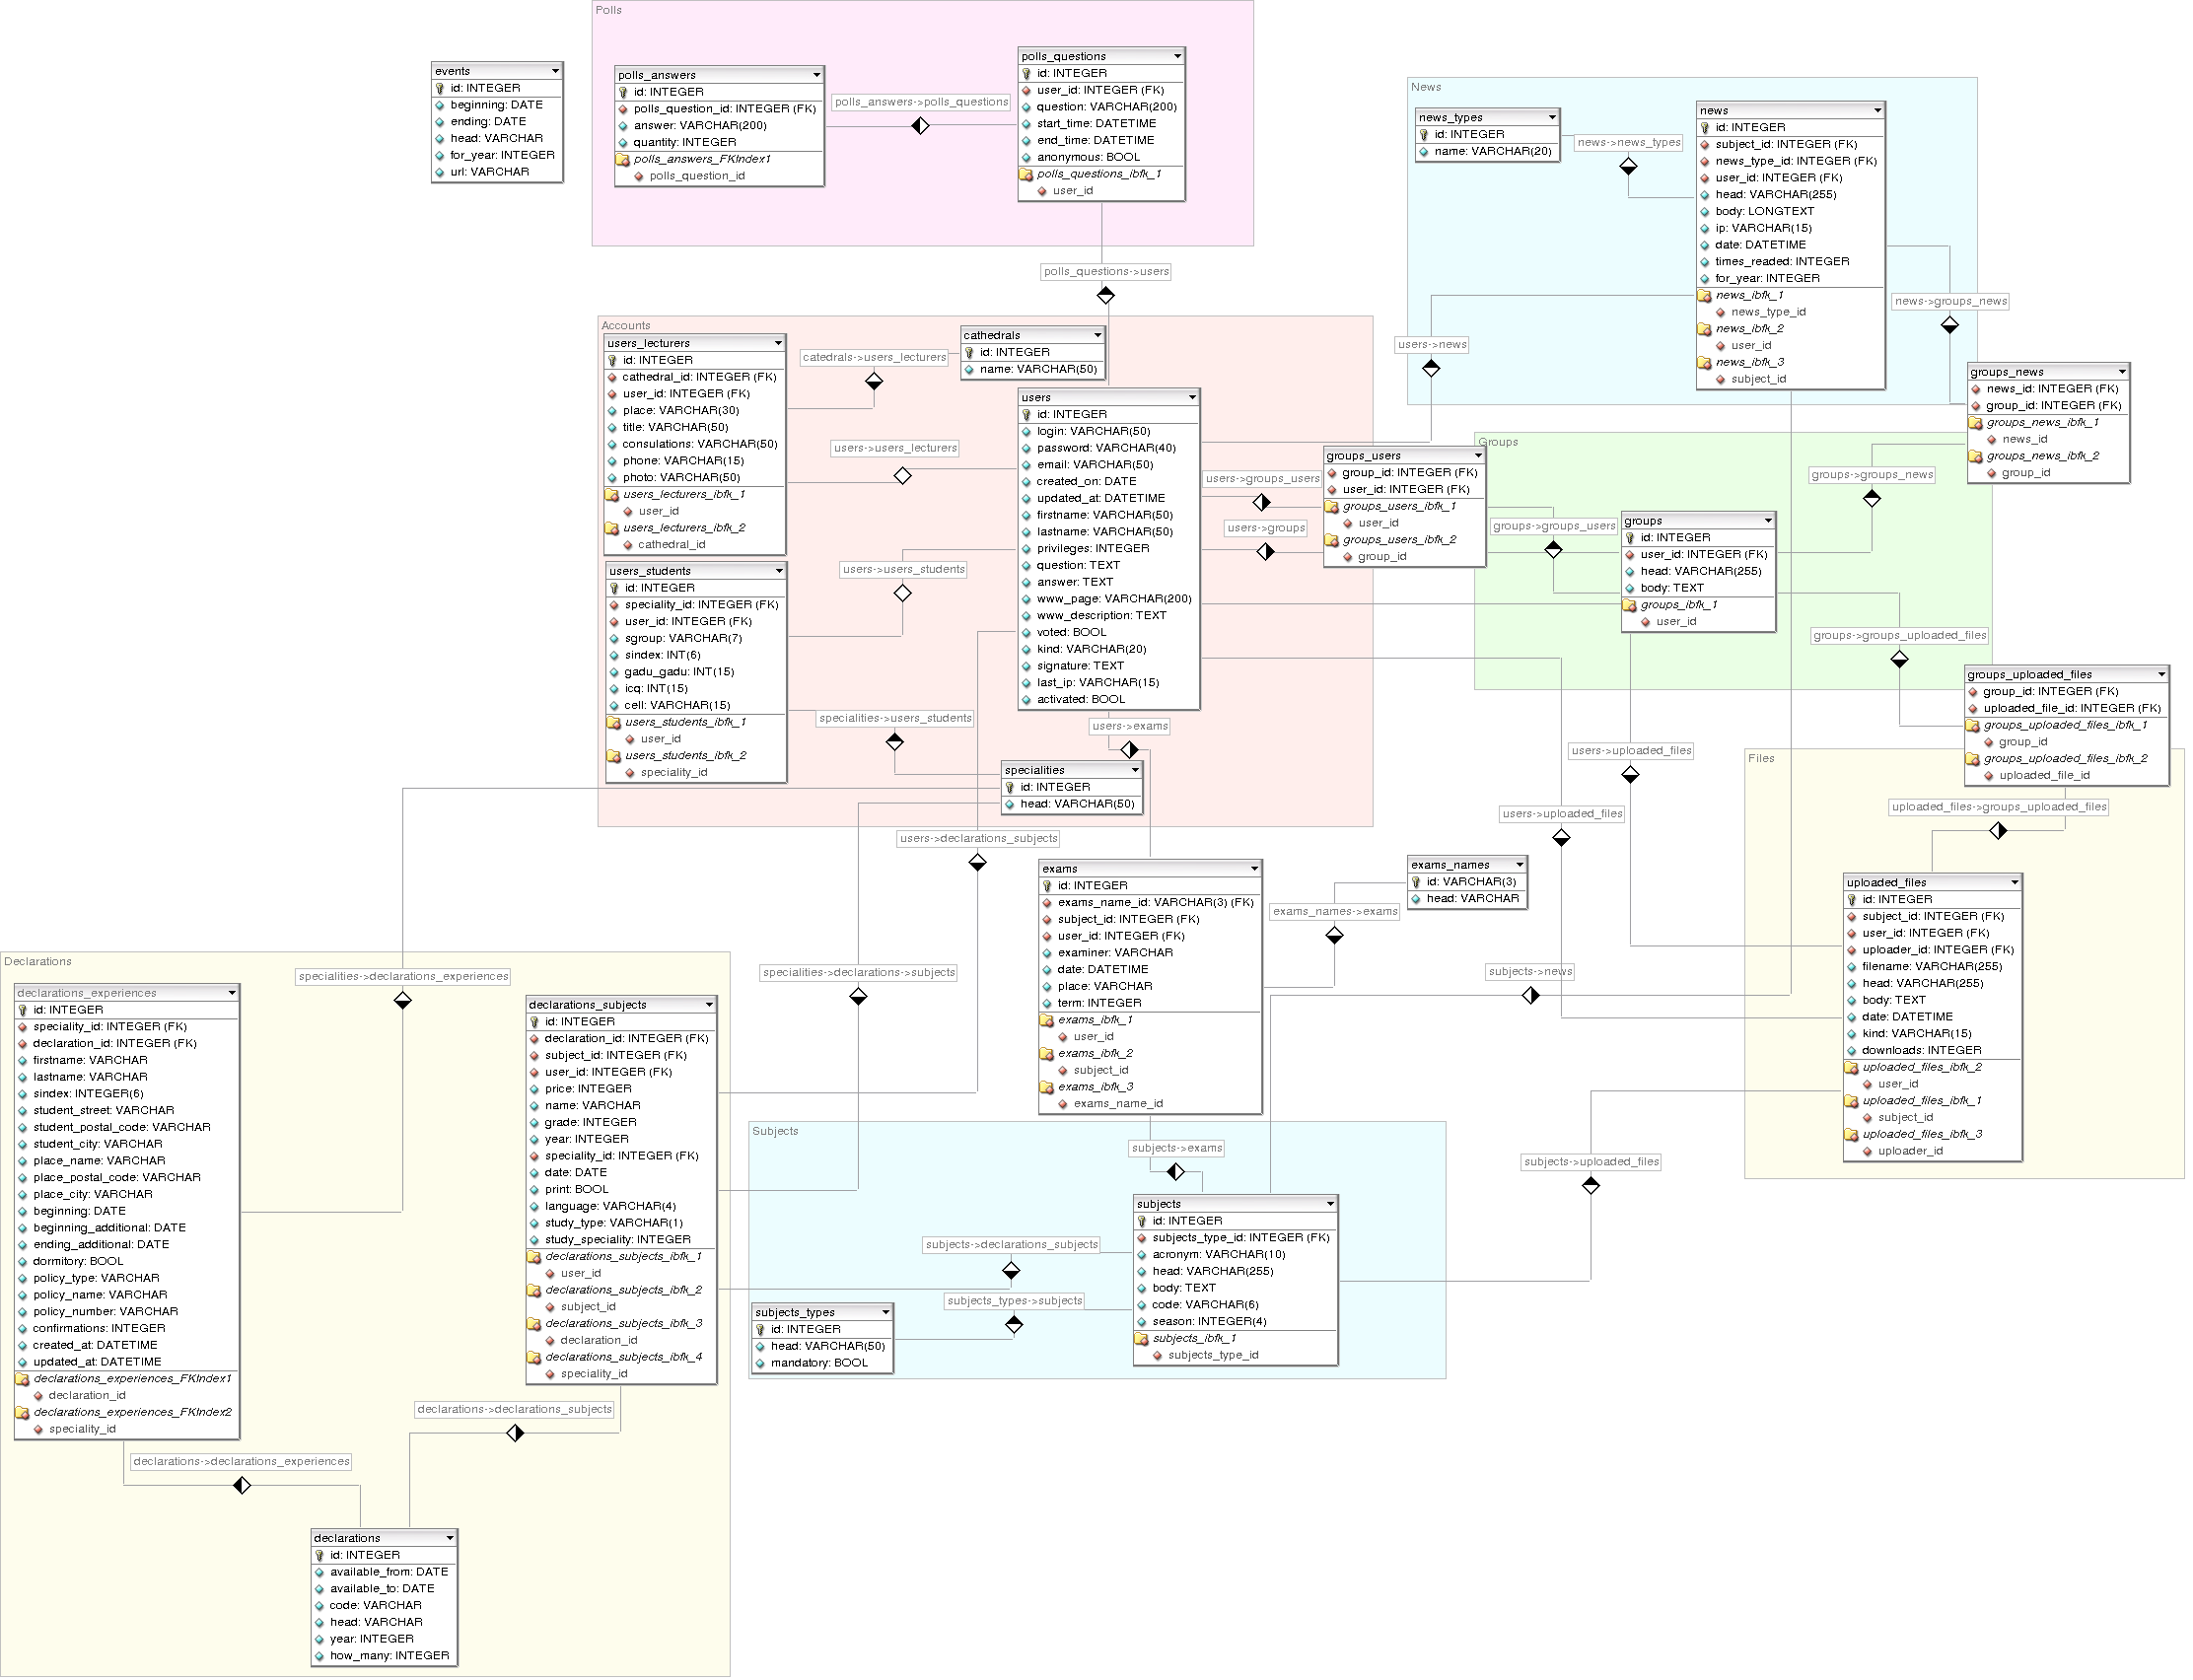
\includegraphics{database.png}
  \caption{
  Schemat bazy danych EiT.
  \label{fig:database}
  }
\end{figure}
\end{landscape}
\newpage

\addtolength{\textwidth}{-4cm}
\addtolength{\hoffset}{2.5cm}
\addtolength{\textheight}{-5cm}
\addtolength{\voffset}{3.5cm}
\subsection{Opis tabel}
\label{sub:tabele}

\subsubsection{Tabela \emph{users}}
\label{subsub:users}

\begin{table}[h]
  \centering
  \begin{tabular}{|c|c|l|}\hline
  Pole & Typ & Opis \\\hline
  id              & int(11)      & \\
  login           & varchar(50)  & login użytkownika \\
  password        & varchar(40)  & hasło użytkownika \\
  email           & varchar(50)  & email użytkownika \\
  created\_on      & date         & data utworzenia konta \\
  updated\_at      & datetime     & data ostatniego zalogowania\\
  firstname       & varchar(50)  & imię \\
  lastname        & varchar(50)  & nazwisko \\
  privileges      & int(11)      & przywileje w systemie \\
  question        & text         & pytanie ratunkowe \\
  answer          & text         & odpowiedź na pytanie ratunkowe \\
  www\_page        & varchar(200) & adres strony WWW użytkownika\\
  www\_description & text         & opis strony WWW \\
  voted           & tinyint(1)   & czy użytkownik zagłosował już w ankiecie? \\
  signature       & text         & sygnaturka użytkownika \\
  last\_ip         & varchar(15)  & ostatnie IP z którego logował się użytkownik \\
  activated       & tinyint(1)   & czy konto jest aktywne? \\\hline
  \end{tabular}
  \caption{Tabela \emph{users}\label{tab:users}}
\end{table}
\begin{figure}[h]
  \centering
  \begin{tabular}{|c|c|c|c|c|c|c|c|}\hline
    X & O & D & A & G & M & K & P \\\hline
  \end{tabular}
  \begin{itemize}
    \item $X_{128}$ -- nieużywany
    \item $O_{64}$ -- dodawanie i edycja ocen
    \item $D_{32}$ -- odczyt deklaracji studenckich
    \item $A_{16}$ -- dodawanie i edycja aktualności
    \item $G_8$ -- konfiguracja grup studentów
    \item $M_4$ -- dodawanie i edycja materiałów
    \item $K_2$ -- konfiguracja wydarzeń w kalendarzu studenckim
    \item $P_1$ -- administracja ankietami
  \end{itemize}
  \caption{Struktura pola \emph{privileges} w tabelce \emph{users}\label{fig:privileges}}
\end{figure}

\begin{itemize}
  \item Tabelka ta zawiera zbiorcze informacje o użytkownikach mogących dostać się do systemu (zarówno studentach, jak i prowadzących).
  \item Pole \emph{login} może być puste. Wraz z początkiem każdego roku akademickiego, dziekanat dostarcza listę nowych studentów. Osoby te są dopisywane do bazy danych. Później, jeśli któraś z nich zapragnie założyć konto, podaje login i hasło, które z miejsca stają się aktywne i włączają użytkownika do systemu. Takie rozwiązanie zapobiega założeniu konta, przez osobę niepowołaną.
  \item Hasło użytkownika jest zahashowane algorytmem SHA-1\footnote{Standard dostępny pod \url{http://csrc.nist.gov/publications/fips/fips180-2/fips180-2withchangenotice.pdf}}. Zabezpiecza to hasła użytkowników przed odczytem w przypadku skompromitowania bazy danych.
  \item Struktura pola \emph{privileges} to maska, w której każdy bit określa inne uprawnienia, jak opisuje to rysunek \ref{fig:privileges}. 1 -- oznacza przyzwolenia, 0 -- brak dostępu
  \item Pola \emph{question} i \emph{answer} nie są obowiązkowe, zabezpieczają jednak użytkownika przed utratą hasła. Po podaniu odpowiedzi na pytanie, użytkownik jest z powrotem logowany do systemu, gdzie może zmienić swoje hasło.
  \item Pole \emph{signature} nie jest nigdzie używane -- zachowano je w celu uzyskania wstecznej zgodności i na poczet przyszłych zastosowań.
\end{itemize}

\subsubsection{Tabela \emph{cathedrals}}
\label{subsub:cathedrals}

\begin{table}[h]
  \centering
  \begin{tabular}{|c|c|l|}\hline
  Pole & Typ & Opis \\\hline
  id              & int(11)      & \\
  name & varchar(50) & Nazwa katedry \\\hline
  \end{tabular}
  \caption{Tabela \emph{cathedrals}\label{tab:cathedrals}}
\end{table}

\begin{itemize}
  \item Tabelka ta zawiera wszystkie katedry obsługiwane przez system.
\end{itemize}

\subsubsection{Tabela \emph{specialities}}
\label{subsub:specialities}

\begin{table}[h]
  \centering
  \begin{tabular}{|c|c|l|}\hline
  Pole & Typ & Opis \\\hline
  id              & int(11)      & \\
  head & varchar(50) & Nazwa specjalności \\\hline
  \end{tabular}
  \caption{Tabela \emph{specialities}\label{tab:specialities}}
\end{table}

\begin{itemize}
  \item Tabelka ta zawiera wszystkie kierunki obsługiwane przez system. Pierwszy wiersz ($id = 1$) jest pusty i zarezerwowany dla studentów, którzy jeszcze nie dokonali wyboru.
\end{itemize}

~\newline

\subsubsection{Tabela \emph{users\_students}}
\label{subsub:users_students}

\begin{table}[h]
  \centering
  \begin{tabular}{|c|c|l|}\hline
  Pole & Typ & Opis \\\hline
  id             & int(11)     & \\
  user\_id       & int(11)     & \\
  speciality\_id & int(11)     & \\
  sgroup         & varchar(7)  & Grupa dziekanatowa\\
  sindex         & int(6)      & Numer indeksu \\
  gadu\_gadu     & int(15)     & Numer Gadu-Gadu \\
  icq            & int(15)     & Numer ICQ \\
  cell           & varchar(15) & Telefon kontaktowy \\\hline

  \end{tabular}
  \caption{Tabela \emph{users\_students}\label{tab:users_students}}
\end{table}

\begin{figure}[h]
  \centering
  \begin{tabular}{|c|c|c|c|}\hline
  K & R & R & S\\\hline
  \end{tabular}
  \begin{itemize}
    \item \emph{K} -- kod kierunku (\emph{E} dla Elektroniki, \emph{K} dla Telekomunikacji)
    \item \emph{RR} -- dwie ostatnie cyfry roku rozpoczęcia studiów przez daną grupę
    \item \emph{S} -- kod specjalności
  \end{itemize}
  \caption{Struktura pola grupy\label{fig:group}}
\end{figure}
\begin{equation}
  rok = \left\{ \begin{array}{ll}
  obecny\_rok - 2000 - RR & gdy~miesiac \le 9\\
  obecny\_rok - 2000 - RR + 1 & gdy~miesiac > 9
  \end{array} \right.
  \label{equ:year}
\end{equation}
\begin{itemize}
  \item Tabelka zawiera informacje o studentach. Prowadzący nie mają w niej rekordów.
  \item \emph{sgroup} i \emph{sindex} mają ,,s'' na początku w związku z obostrzeniami MySQL (\emph{index} i \emph{group} są słowami zastrzeżonymi).
  \item Na podstawie grupy dziekanatowej, obliczany jest rok studiów wg. wzoru \ref{equ:year}
\end{itemize}

\newpage
\subsubsection{Tabela \emph{users\_lecturers}}
\label{subsub:users_lecturers}

\begin{table}[h]
  \centering
  \begin{tabular}{|c|c|l|}\hline
  Pole & Typ & Opis \\\hline
  id            & int(11)     & \\
  cathedral\_id & int(11)     & \\
  user\_id      & int(11)     & \\
  place         & varchar(30) & Pokój \\
  title         & varchar(50) & Tytuł naukowy \\
  consultations & varchar(50) & Terminy konsultacji \\
  phone         & varchar(15) & Telefon kontaktowy \\
  photo         & varchar(50) & Zdjęcie \\\hline
  \end{tabular}
  \caption{Tabela \emph{users\_lecturers}\label{tab:users_lecturers}}
\end{table}
\begin{itemize}
  \item Tabelka zawiera informacje o prowadzących. Studenci nie są do niej dopisywani.
  \item Pole \emph{photo} zawiera tylko nazwę pliku ze zdjęciem. Model w aplikacji sam ustala ścieżkę.
\end{itemize}

\subsubsection{Tabela \emph{subjects\_types}}
\label{subsub:subjects_types}

\begin{table}[h]
  \centering
  \begin{tabular}{|c|c|l|}\hline
  Pole & Typ & Opis \\\hline
  id        & int(11)     & \\
  head      & varchar(50) & Nazwa rodzaju \\
  mandatory & tinyint(1)  & Czy obowiązkowy? \\\hline
  \end{tabular}
  \caption{Tabela \emph{subjects\_types}\label{tab:subjects_types}}
\end{table}
\begin{itemize}
  \item Tabelka zawiera kategorie (rodzaje) przedmiotów. Istotne przy grupowaniu po kategoriach.
\end{itemize}

\newpage
\subsubsection{Tabela \emph{subjects}}
\label{subsub:subjects}

\begin{table}[h]
  \centering
  \begin{tabular}{|c|c|l|}\hline
  Pole & Typ & Opis \\\hline
  id                 & int(11)      & \\
  subjects\_type\_id & int(11)      & \\
  acronym            & varchar(10)  & Skrót nazwy przedmiotu\\
  head               & varchar(255) & Nazwa przedmiotu \\
  body               & text         & Opis przedmiotu \\
  code               & varchar(6)   & Kod dziekanatowy \\
  season             & int(4)       & Semestr \\\hline
  \end{tabular}
  \caption{Tabela \emph{subjects}\label{tab:subjects}}
\end{table}
\begin{itemize}
  \item Tabelka zawiera informacje o wykładanych przedmiotach. Przedmiot liczy się jako całość (nie ma podziału na wykłady, laboratoria etc.)
  \item Pole \emph{season} oznacz semestr na którym dany przedmiot jest prowadzony. Jeśli wynosi 0, oznacza to przedmiot specjalny (np. Dziekanat).
\end{itemize}

\subsubsection{Tabela \emph{news\_types}}
\label{subsub:news_types}

\begin{table}[h]
  \centering
  \begin{tabular}{|c|c|l|}\hline
  Pole & Typ & Opis \\\hline
  id              & int(11)      & \\
  name & varchar(20) & Rodzaj aktualności \\\hline
  \end{tabular}
  \caption{Tabela \emph{news\_types}\label{tab:news_types}}
\end{table}

\begin{itemize}
  \item Tabelka ta zawiera kategorie aktualności.
\end{itemize}

\newpage
\subsubsection{Tabela \emph{news}}
\label{subsub:news}

\begin{table}[h]
  \centering
  \begin{tabular}{|c|c|l|}\hline
  Pole & Typ & Opis \\\hline
  id             & int(11)      & \\
  news\_type\_id & int(11)      & \\
  user\_id       & int(11)      & \\
  subject\_id    & int(11)      & \\
  head           & varchar(255) & Tytuł aktualności \\
  body           & text         & Treść aktualności \\
  ip             & varchar(15)  & IP z której dodano aktualność \\
  date           & datetime     & Data dodania \\
  times\_readed  & int(11)      & Ilość przeczytań \\
  for\_year      & int(11)      & Dla których lat \\\hline
  \end{tabular}
  \caption{Tabela \emph{news}\label{tab:news}}
\end{table}

\begin{itemize}
  \item Tabelka ta zawiera aktualności.
  \item Pole \emph{for\_year} to maska roczników których dotyczy aktualność, przy czym najmłodszy bit to pierwszy rok, najstarszy -- piąty. Jeżeli pole ma wartość ,,0'' to aktualność dotyczy wszystkich.
\end{itemize}

\subsubsection{Tabela \emph{uploaded\_files}}
\label{subsub:uploaded_files}

\begin{table}[h]
  \centering
  \begin{tabular}{|c|c|l|}\hline
  Pole & Typ & Opis \\\hline
  id           & int(11)      & \\
  subject\_id  & int(11)      & \\
  user\_id     & int(11)      & \\
  uploader\_id & int(11)      & \\
  filename     & varchar(255) & Nazwa pliku \\
  head         & varchar(255) & Tytuł pliku \\
  body         & text         & Opis pliku \\
  date         & datetime     & Data dodania \\
  kind         & varchar(15)  & Rodzaj \\
  downloads    & int(11)      & Ilość pobrań \\\hline
  \end{tabular}
  \caption{Tabela \emph{uploaded\_files}\label{tab:uploaded_files}}
\end{table}

\begin{itemize}
  \item Tabelka ta zawiera informacje o plikach wgranych do systemu (materiałach lub ocenach). Jest także tabelką pośredniczącą dla relacji wiele-do-wielu między prowadzącymi a przedmiotami (zob. rozdz.~\ref{rel:subjects_users}, str.~\pageref{rel:subjects_users}).
  \item Pole \emph{filename} zawiera tylko nazwę pliku. System sam określi ścieżkę.
  \item Pole \emph{kind} określa rodzaj pliku. Możliwe są dwa stany:
  \begin{itemize}
    \item \emph{material} -- plik z materiałami,
    \item \emph{grade} -- plik z ocenami.
  \end{itemize}
\end{itemize}

\subsubsection{Tabela \emph{groups}}
\label{subsub:groups}

\begin{table}[h]
  \centering
  \begin{tabular}{|c|c|l|}\hline
  Pole & Typ & Opis \\\hline
  id       & int(11)      & \\
  user\_id & int(11)      & \\
  head     & varchar(255) & Nazwa grupy \\
  body     & text         & Opis grupy \\\hline
  \end{tabular}
  \caption{Tabela \emph{groups}\label{tab:groups}}
\end{table}
\begin{itemize}
  \item Tabelka zawiera grupy użytkowników. Podstawowe typy grup to:
  \begin{itemize}
    \item Administratorzy,
    \item Zalogowani,
    \item Specjalności (Elektronik, Telekomunikacja),
    \item Lata (Rok I -- Rok V),
    \item Grupy dziekanatowe (1 -- 10).
  \end{itemize}
  \item Każdy prowadzący może dodawać swoje grupy.
  \item Grupy pełnią istotną rolę przy określaniu uprawnień do plików, dzięki nim możliwe jest dodawanie materiałów np. tylko dla III roku albo tylko dla Elektroniki.
\end{itemize}

\newpage
\subsubsection{Tabela \emph{polls\_questions}}
\label{subsub:polls_questions}

\begin{table}[h]
  \centering
  \begin{tabular}{|c|c|l|}\hline
  Pole & Typ & Opis \\\hline
  id          & int(11)      & \\
  user\_id    & int(11)      & \\
  question    & varchar(200) & Pytanie \\
  start\_time & datetime     & Czas rozpoczęcia \\
  end\_time   & datetime     & Czas zakończenia \\
  anonymous   & tinyint(1)   & Czy anonimowa? \\\hline

  \end{tabular}
  \caption{Tabela \emph{polls\_questions}\label{tab:polls_questions}}
\end{table}
\begin{itemize}
  \item Tabelka zawiera informacje o ankietach wraz z pytaniem.
  \item Pole \emph{question} zawiera pytanie, jakie będzie zadane w ankiecie.
  \item Pole \emph{end\_time} określa czas zakończenia ankiety. Po jego upływie, ankieta zostaje automatycznie zamknięta. Jeśli pozostanie puste, ankieta jest bezterminowa.
  \item Pole \emph{anonymous} informuja czy ankieta jest anonimowa. Na stronie maksymalnie mogą być aktywne naraz dwie ankiety -- jedna anonimowa, druga nie.
\end{itemize}

\subsubsection{Tabela \emph{polls\_answers}}
\label{subsub:polls_answers}

\begin{table}[h]
  \centering
  \begin{tabular}{|c|c|l|}\hline
  Pole & Typ & Opis \\\hline
  id          & int(11)      & \\
  polls\_question\_id & int(11)      & \\
  answer              & varchar(200) & Odpowiedź \\
  quantity            & int(11)      & Ilość udzieleń \\\hline
  \end{tabular}
  \caption{Tabela \emph{polls\_answers}\label{tab:polls_answers}}
\end{table}
\begin{itemize}
  \item Tabelka zawiera odpowiedzi do pytań zadanych w ankietach. Jedna ankieta może mieć maksymalnie sześć odpowiedzi (baza tego nie sprawdza).
  \item Pole \emph{quantity} zawiera ilość użytkowników którzy wybrali tą odpowiedź. Na podstawie tego pola, później jest liczony procentowy udział tego wyboru.
\end{itemize}

\newpage

\subsubsection{Tabela \emph{exams\_names}}
\label{subsub:exams_names}

\begin{table}[h]
  \centering
  \begin{tabular}{|c|c|l|}\hline
  Pole & Typ & Opis \\\hline
  id   & varchar(3)   & Kod \\
  head & varchar(255) & Nazwa \\\hline
  \end{tabular}
  \caption{Tabela \emph{exams\_names}\label{tab:exams_names}}
\end{table}

\begin{itemize}
  \item Tabelka ta zawiera nazwy odpowiednich kombinacji typu studiów, roku i kierunku przyporządkowane do ich kodu.
  \item Pole \emph{id} wyjątkowo nie jest tu wartością liczbową, a kombinacją trzech znaków. Jest jednak jednoznacznie identyfikowalne i ma odnoszący się do niego klucz obcy w tabeli \emph{exams}.
\end{itemize}

\subsubsection{Tabela \emph{exams}}
\label{subsub:exams}

\begin{table}[h]
  \centering
  \begin{tabular}{|c|c|l|}\hline
  Pole & Typ & Opis \\\hline
  id   & int(11)   &  \\
  subject\_id     & int(11)      & \\
  user\_id        & int(11)      & \\
  exams\_name\_id & varchar(3)   & \\
  examiner        & varchar(255) & Dane egzaminatora \\
  date            & datetime     & Data egzaminu \\
  place           & varchar(255) & Miejsce egzaminu \\
  term            & int(11)      & Termin \\\hline

  \end{tabular}
  \caption{Tabela \emph{exams}\label{tab:exams}}
\end{table}

\begin{itemize}
  \item Tabelka ta zawiera informacje o egzaminach w najbliższej sesji.
  \item Pole \emph{examiner} zawiera dane egzaminatora wpisane na sztywno, a nie referencję do odpowiedniego rekordu. Bierze się to stąd, że czasami egzamin może przeprowadzać osoba spoza katedry.
  \item Pole \emph{term} określa termin egzaminy i powinno zawierać się w przedziale <0;3>.
\end{itemize}

\newpage
\subsubsection{Tabela \emph{events}}
\label{subsub:events}

\begin{table}[h]
  \centering
  \begin{tabular}{|c|c|l|}\hline
  Pole & Typ & Opis \\\hline
  id   & int(11)   & \\
  beginning  & date         & Początek \\
  ending     & date         & Koniec \\
  head       & varchar(255) & Opis \\
  for\_year  & int(11)      & Dla których lat \\
  url        & varchar(255) & Link \\\hline
  \end{tabular}
  \caption{Tabela \emph{events}\label{tab:events}}
\end{table}

\begin{itemize}
  \item Tabelka ta zawiera kalendarz studenta.
  \item Pole \emph{for\_year} funkcjonuje na identycznej zasadzie, jak to z tabelki \emph{news} (zob. rozdz.~\ref{subsub:news}, str.~\ref{subsub:news}).
  \item Pole \emph{url} nie jest obowiązkowe. Jeśli jednak zostanie podane, cały tytuł będzie linkiem do podanego w \emph{url} adresu.
\end{itemize}

\subsubsection{Tabela \emph{declarations}}
\label{subsub:declarations}

\begin{table}[h]
  \centering
  \begin{tabular}{|c|c|l|}\hline
  Pole & Typ & Opis \\\hline
  id   & int(11)   & \\
  available\_from & date         & Dostępna od... \\
  available\_to   & date         & Dostępna do... \\
  code            & varchar(255) & Kod deklaracji \\
  head            & varchar(255) & Nazwa deklaracji \\
  year            & int(11)      & Dla którego roku \\
  how\_many       & int(11)      & Ile opcji \\\hline

  \end{tabular}
  \caption{Tabela \emph{declarations}\label{tab:declarations}}
\end{table}

\begin{itemize}
  \item Tabelka ta zawiera informacje o samych deklaracjach jako takich. Nie zawiera informacji o wyborach dokonanych przez studentów.
  \item Pola \emph{available\_from} i \emph{available\_to} zawierają przedział czasowy w którym dana deklaracja jest dostępna do wypełnienia. Rok nie jest brany pod uwagę.
  \item Pole \emph{year} określa, którego roku akademickiego taka deklaracja dotyczy. Nie działa tu mechanizm znany z \emph{for\_year} -- jedna deklaracja jest tylko dla jednego roku.
  \item Pole \emph{how\_many} dotyczy tylko deklaracji odnoszących się do wyboru przedmiotów obieralnych. Jest to liczba dwucyfrowa. Liczba dziesiątek oznacza ilość przedmiotów dla Elektroniki, jedności -- dla Telekomunikacji.
\end{itemize}

\subsubsection{Tabela \emph{declarations\_subjects}}
\label{subsub:declarations_subjects}

\begin{table}[h]
  \centering
  \begin{tabular}{|c|c|l|}\hline
  Pole & Typ & Opis \\\hline
  id   & int(11)   & \\
  declaration\_id   & int(11)      & \\
  subject\_id       & int(11)      & \\
  user\_id          & int(11)      & \\
  price             & int(11)      & Cena materiałów \\
  name              & varchar(255) & Nazwa po angielsku \\
  grade             & decimal(2,1) & Ocena \\
  year              & int(11)      & Rok rozpoczęcia studiów \\
  speciality\_id    & int(11)      & Kierunek \\
  date              & date         & Data złożenia \\
  language          & varchar(4)   & Język przedmiotu \\
  print             & tinyint(1)   & Drukować materiały? \\
  study\_type       & varchar(1)   & Typ studiów \\
  study\_speciality & int(11)      & Specjalność \\\hline
  \end{tabular}
  \caption{Tabela \emph{declarations\_subjects}\label{tab:declarations_subjects}}
\end{table}

\begin{itemize}
  \item Tabelka ta zawiera szczegółowe informacje o deklaracjach, a także informacje wypełniane przez studentów. Tabelkę tę można dowolnie modyfikować. Więcej na ten temat zostało przedstawione w dziale Deklaracje (zob. rozdz.~\ref{sub:deklaracje}, str.~\ref{sub:deklaracje}).
  \item Pole \emph{price} dotyczy tylko deklaracji dotyczących druku materiałów. Oznacza ona cenę materiałów w złotówkach pomnożoną przez 10. Nie wypełniają go studenci.
  \item Pole \emph{name} dotyczy tylko deklaracji wyboru języka przedmiotów. Zawiera angielski odpowiednik nazwy przedmiotu. Nie wypełniają go studenci.
  \item Pole \emph{grade} dotyczy tylko deklaracji wyboru kierunku studiów. Oznacza ono ocenę z danego przedmiotu. Jest wypełniane przez studentów. Dodatkowo model oferuje metodę \emph{average}, która obliczą średnią ocen danego studenta.
  \item Pole \emph{year} dotyczy tylko deklaracji wyboru kierunku studiów. Oznacza ono rok, w którym dany student rozpoczął studiowanie na Elektronice i Telekomunikacji. Jest wypełniane przez studentów.
  \item Pole \emph{speciality\_id} dotyczy tylko deklaracji wyboru kierunku studiów. Zawiera id kierunku (referencja do specialities) na którym dany student chciałby kontynuuować swoją edukację. Jest wypełniane przez studentów.
  \item Pole \emph{date} zawiera dotyczy wszystkich deklaracji. Zawiera datę ich złożenia. Jest wypełniane przez system automatycznie.
  \item Pole \emph{language} dotyczy tylko deklaracji wyboru języka przedmiotów. Zawiera dwuliteroww kody języków wybrane przez studenta w formacie WWDD, gdzie WW to kod dla wykładu, a DD to kod dla zajęc dodatkowych (laboratoriów, ćwiczeń, etc.). Jest wypełniane przez studentów.
  \item Pole \emph{print} dotyczy tylko deklaracji dotyczących druku materiałów. Jeśli jest ustawione na 1, oznacza, że dany student życzy sobie materiały w formie papierowej dla danego przedmiotu. Jest wypełniane przez studentów.
  \item Pole \emph{study\_type} dotyczy tylko deklaracji wyboru specjalności. Określa ono rodzaj studiów -- M to studia magisterskie, I to studia inżynierskie. Jest wypełniane przez studentów.
  \item Pole \emph{study\_speciality} dotyczy tylko deklaracji wyboru specjalności. Zawiera ono cyfrowy kod specjalności. Jest wypełniane przez studentów.
\end{itemize}

\newpage
\subsubsection{Tabela \emph{declarations\_experiences}}
\label{subsub:declarations_experiences}

\begin{table}[h]
  \centering
  \begin{tabular}{|c|c|l|}\hline
  Pole & Typ & Opis \\\hline
  id   & int(11)   & \\
  declaration\_id       & int(11)      & \\
  firstname             & varchar(255) & Imię studenta \\
  lastname              & varchar(255) & Nazwisko studenta \\
  sindex                & int(6)       & Numer indeksu \\
  speciality\_id        & int(11)      & \\
  student\_street       & varchar(255) & Adres zamieszkania \\
  student\_postal\_code & varchar(255) & Kod pocztowy\\
  student\_city         & varchar(255) & Miasto \\
  place\_name           & varchar(255) & Miejsce praktyki \\
  place\_street         & varchar(255) & Adres zakładu pracy \\
  place\_postal\_code   & varchar(255) & Kod pocztowy\\
  place\_city           & varchar(255) & Miasto \\
  beginning             & date         & Termin rozpoczęcia \\
  beginning\_additional & date         & Dodatkowy termin \\
  ending\_additional    & date         & Koniec dodatkowego terminu \\
  dormitory             & tinyint(1)   & Czy chce akademik? \\
  policy\_type          & varchar(255) & Rodzaj ubezpieczenia \\
  policy\_name          & varchar(255) & Nazwa polisy \\
  policy\_number        & varchar(255) & Numer polisy \\
  confirmations         & int(11)      & Potwierdzenia \\
  created\_at           & datetime     & Utworzono \\
  updated\_at           & datetime     & Poprawiono \\\hline
  \end{tabular}
  \caption{Tabela \emph{declarations\_experiences}\label{tab:declarations_experiences}}
\end{table}

\begin{figure}[h]
  \centering
  \begin{tabular}{|c|c|c|c|c|}\hline
  E & D & C & B & A \\\hline
  \end{tabular}
  \begin{itemize}
    \item A -- dostarczone zaświadczenie z miejsca praktyki
    \item B -- dostarczona informacja o ubezpieczeniu
    \item C -- dostarczone potwierdzenie odbycia praktyki i sprawozdanie
    \item D -- praktyka bezpłatna
    \item E -- wpis do indeksu
  \end{itemize}
  \caption{Struktura pola \emph{confirmations}\label{fig:confirmations}}
\end{figure}

\begin{itemize}
  \item Tabelka ta zawiera szczegółowe informacje dotyczące praktyki zawodowej danego studenta.
  \item Pola \emph{student\_street}, \emph{student\_postal\_code}, \emph{student\_city} dotyczą adresu zameldowania studenta.
  \item Pola \emph{place\_name}, \emph{place\_street}, \emph{place\_postal\_code}, \emph{pace\_city} dotyczą informacji o zakładzie pracy, w którym będzie odbywać się praktyka.
  \item Pole \emph{beginning} to termin rozpoczęcia praktyki.
  \item Pola \emph{beginning\_additional} i \emph{ending\_additional} określają dodatkowy termin praktyki, w przypadku gdyby praktyka była dwuetapowa.
  \item Pole \emph{dormitory} określa, czy student jest zainteresowany pobytem w akademiku na czas praktyki.
  \item Pola \emph{policy\_type}, \emph{policy\_name} i \emph{policy\_number} dotyczą obowiązkowego dokumentu, potwierdzającego ubezpieczenie na czas praktyki.
  \item Pole \emph{confirmations} zawiera potwierdzenia dla opiekuna praktyk, a jego struktura została przedstawiona na ryskunku \ref{fig:confirmations}.
\end{itemize}


\subsection{Opis relacji}
\label{sub:relacje}

\subsubsection{Relacja \emph{users}$\to$\emph{users\_students}}
\label{subsub:users-users_students}
\begin{itemize}
  \item Typ relacji: 1 do 1
  \item Pole: \emph{users\_students}.\emph{user\_id}
  \item Klucz obcy: \emph{users\_students\_ibfk\_1}
  \item Obowiązkowa
  \item Dodaje dodatkowe informacje o studencie, specyficzne tylko dla niego.
\end{itemize}

\subsubsection{Relacja \emph{specialities}$\to$\emph{users\_students}}
\label{subsub:specialities-users_students}
\begin{itemize}
  \item Typ relacji: 1 do wielu
  \item Pole: \emph{users\_students}.\emph{speciality\_id}
  \item Klucz obcy: \emph{users\_students\_ibfk\_2}
  \item Obowiązkowa
  \item Informacje o kierunku studiów studenta. Jeśli jeszcze nie został wybrany, pole przyjmuje wartość 1 (zob. tab.~\ref{subsub:specialities}, str.~\pageref{subsub:specialities}).
\end{itemize}

\subsubsection{Relacja \emph{cathedrals}$\to$\emph{users\_lecturers}}
\label{subsub:cathedrals-users_lecturers}
\begin{itemize}
  \item Typ relacji: 1 do wielu
  \item Pole: \emph{users\_lecturers}.\emph{cathedral\_id}
  \item Klucz obcy: \emph{users\_lecturers\_ibfk\_1}
  \item Obowiązkowa
  \item Katedra do której dany prowadzący należy.
\end{itemize}

\subsubsection{Relacja \emph{users}$\to$\emph{users\_lecturers}}
\label{subsub:users-users_lecturers}
\begin{itemize}
  \item Typ relacji: 1 do 1
  \item Pole: \emph{users\_lecturers}.\emph{user\_id}
  \item Klucz obcy: \emph{users\_lecturers\_ibfk\_2}
  \item Obowiązkowa
  \item Dodatkowe informacje o prowadzącym, specyficzne tylko dla niego.
\end{itemize}

\subsubsection{Relacja \emph{subjects\_types}$\to$\emph{subjects}}
\label{subsub:subjects_types-subjects}
\begin{itemize}
  \item Typ relacji: 1 do wielu
  \item Pole: \emph{subjects}.\emph{subjects\_type\_id}
  \item Klucz obcy: \emph{subjects\_ibfk\_1}
  \item Nieobowiązkowa
  \item Informacje o rodzaju danego przedmiotu.
\end{itemize}

\subsubsection{Relacja \emph{users}$\leftrightarrow$\emph{subjects}}
\label{subsub:users-subjects}
\begin{itemize}
  \item Typ relacji: wiele do wielu
  \item Pola: \emph{uploaded\_files}.\emph{user\_id}, \emph{uploaded\_files}.\emph{subject\_id}
  \item Tabelka pośrednicząca: \emph{uploaded\_files}
  \item Klucze obce: \emph{uploaded\_files\_ibfk\_1}, \emph{uploaded\_files\_ibfk\_2}
  \item Obowiązkowa
  \item Relacja wykorzystywana do określenia, które przedmioty prowadzi jaki wykładowca. Aby uniknąć z każdym semestrem ręcznego ich dodawania, wszystko dzieje automatycznie. Kryterium bycia prowadzącym, jest dodanie pliku do systemu i przypisanie siebie jak prowadzącego do określonego przedmiotu. Wtedy taka osoba (oczywiście, jeśli dodatkowo jest wykładowcą, czyli jest wpisana do tabelki \emph{users\_lecturers}) automatycznie tworzy sobie relację z tym przedmiotem poprzez tabelkę \emph{uploaded\_files}, co system odczytuje również jako prowadzenie tychże zajęć.
\end{itemize}

\subsubsection{Relacja \emph{news\_types}$\to$\emph{news}}
\label{subsub:news_types-news}
\begin{itemize}
  \item Typ relacji: 1 do wielu
  \item Pole: \emph{news}.\emph{news\_type\_id}
  \item Klucz obcy: \emph{news\_ibfk\_1}
  \item Nieobowiązkowa
  \item Informacje o rodzaju aktualności. Obecnie niewykorzystywane. Zachowane dla wstecznej zgodności i na poczet przyszłych zastosowań.
\end{itemize}

\subsubsection{Relacja \emph{users}$\to$\emph{news}}
\label{subsub:users-news}
\begin{itemize}
  \item Typ relacji: 1 do wielu
  \item Pole: \emph{news}.\emph{user\_id}
  \item Klucz obcy: \emph{news\_ibfk\_2}
  \item Obowiązkowa
  \item Określa autora danej aktualności.
\end{itemize}

\subsubsection{Relacja \emph{subjects}$\to$\emph{news}}
\label{subsub:subjects-news}
\begin{itemize}
  \item Typ relacji: 1 do wielu
  \item Pole: \emph{news}.\emph{subject\_id}
  \item Klucz obcy: \emph{news\_ibfk\_3}
  \item Nieobowiązkowa
  \item Określa przedmiot, którego dotyczy dana aktualność.
\end{itemize}

\subsubsection{Relacja \emph{users}$\to$\emph{uploaded\_files}}
\label{subsub:users-uploaded_files}
\begin{itemize}
  \item Typ relacji: 1 do wielu
  \item Pole: \emph{uploaded\_files}.\emph{uploader\_id}
  \item Klucz obcy: \emph{uploaded\_files\_ibfk\_3}
  \item Obowiązkowa
  \item Informacja o tym kto dodał dany plik dla danego przedmiotu. Nie jest to jednoznaczne z byciem prowadzącym. Podczas dodawania pliku, można określić, kto prowadzi dany przedmiot i może to być osoba inna od osoby dodającej plik.
\end{itemize}

\subsubsection{Relacja \emph{users}$\to$\emph{groups}}
\label{subsub:users-groups}
\begin{itemize}
  \item Typ relacji: 1 do wielu
  \item Pole: \emph{groups}.\emph{user\_id}
  \item Klucz obcy: \emph{groups\_ibfk\_1}
  \item Nieobowiązkowa
  \item Informacja kto jest właścicielem danej grupy.
\end{itemize}

\subsubsection{Relacja \emph{groups}$\leftrightarrow$\emph{users}}
\label{subsub:groups-users}
\begin{itemize}
  \item Typ relacji: wiele do wielu
  \item Tabelka pośrednicząca: \emph{groups\_users}
  \item Pola: \emph{groups\_users}.\emph{group\_id}, \emph{groups\_users}.\emph{user\_id}
  \item Klucze obce: \emph{groups\_users\_ibfk\_1}, \emph{groups\_users\_ibfk\_2}
  \item Obowiązkowa
  \item Informacje o przypisaniu użytkowników do grup.
\end{itemize}

\subsubsection{Relacja \emph{groups}$\leftrightarrow$\emph{news}}
\label{subsub:groups-news}
\begin{itemize}
  \item Typ relacji: wiele do wielu
  \item Tabelka pośrednicząca: \emph{groups\_news}
  \item Pola: \emph{groups\_news}.\emph{group\_id}, \emph{groups\_news}.\emph{news\_id}
  \item Klucze obce: \emph{groups\_news\_ibfk\_1}, \emph{groups\_news\_ibfk\_2}
  \item Obowiązkowa
  \item Informacje o uprawnieniach do odczytu określonych wiadomości przez grupy. W starym systemie funkcjonalność praktycznie nieużywana. W nowym porzucona, zachowana tylko na poczet przyszłych ustaleń.
\end{itemize}

\subsubsection{Relacja \emph{groups}$\leftrightarrow$\emph{uploaded\_files}}
\label{subsub:groups-uploaded_files}
\begin{itemize}
  \item Typ relacji: wiele do wielu
  \item Tabelka pośrednicząca: \emph{groups\_uploaded\_files}
  \item Pola: \emph{groups\_uploaded\_files}.\emph{group\_id}, \emph{groups\_uploaded\_files}.\emph{uploaded\_file\_id}
  \item Klucze obce: \emph{groups\_uploaded\_files\_ibfk\_1}, \emph{groups\_uploaded\_files\_ibfk\_2}
  \item Obowiązkowa
  \item Uprawnienia grup do określonych plików. Bardzo ważna funkcjonalność, która zabezpiecza np. materiały dla studentów określonego roku, przed ściągnięciem ich przez studentów innych lat.
\end{itemize}

\subsubsection{Relacja \emph{users}$\to$\emph{polls\_questions}}
\label{subsub:users-polls_questions}
\begin{itemize}
  \item Typ relacji: 1 do wielu
  \item Pole: \emph{polls\_questions}.\emph{user\_id}
  \item Klucz obcy: \emph{polls\_questions\_ibfk\_1}
  \item Obowiązkowa
  \item Określa autora ankiety.
\end{itemize}

\subsubsection{Relacja \emph{polls\_questions}$\to$\emph{polls\_answers}}
\label{subsub:polls_questions-polls_answers}
\begin{itemize}
  \item Typ relacji: 1 do wielu
  \item Pole: \emph{polls\_answers}.\emph{polls\_question\_id}
  \item Klucz obcy: \emph{polls\_answers\_ibfk\_1}
  \item Obowiązkowa
  \item Przypisuje daną odpowiedź do określonej ankiety.
\end{itemize}

\subsubsection{Relacja \emph{subjects}$\to$\emph{exams}}
\label{subsub:subjects-exams}
\begin{itemize}
  \item Typ relacji: 1 do wielu
  \item Pole: \emph{exams}.\emph{subject\_id}
  \item Klucz obcy: \emph{exams\_ibfk\_1}
  \item Obowiązkowa
  \item Przedmiot z którego odbędzie się egzamin.
\end{itemize}

\subsubsection{Relacja \emph{users}$\to$\emph{exams}}
\label{subsub:users-exams}
\begin{itemize}
  \item Typ relacji: 1 do wielu
  \item Pole: \emph{exams}.\emph{user\_id}
  \item Klucz obcy: \emph{exams\_ibfk\_2}
  \item Obowiązkowa
  \item Osoba, która dodała informację o egzaminie.
\end{itemize}

\subsubsection{Relacja \emph{exams\_names}$\to$\emph{exams}}
\label{subsub:exams_names-exams}
\begin{itemize}
  \item Typ relacji: 1 do wielu
  \item Pole: \emph{exams}.\emph{exams\_name\_id}
  \item Klucz obcy: \emph{exams\_ibfk\_3}
  \item Obowiązkowa
  \item Specyficzna relacja, gdyż kluczem obcym nie jest tu liczba a trzyznakowy kod. Kod ten to kombinacja typu studiów, roku i kierunku studiów. Wszystkie egzaminy w systemie są pogrupowane wg. tych kodów, a te relacja służy ich rozwinięciu na pełną nazwę.
\end{itemize}

\subsubsection{Relacja \emph{declarations}$\to$\emph{declarations\_subjects}}
\label{subsub:declarations-declarations_subjects}
\begin{itemize}
  \item Typ relacji: 1 do wielu
  \item Pole: \emph{declarations\_subjects}.\emph{declaration\_id}
  \item Klucz obcy: \emph{declrations\_subjects\_ibfk\_1}
  \item Obowiązkowa
  \item Relacja przypisująca parametry, danej deklaracji.
\end{itemize}

\subsubsection{Relacja \emph{subjects}$\to$\emph{declarations\_subjects}}
\label{subsub:subjects-declarations_subjects}
\begin{itemize}
  \item Typ relacji: 1 do wielu
  \item Pole: \emph{declarations\_subjects}.\emph{subject\_id}
  \item Klucz obcy: \emph{declrations\_subjects\_ibfk\_2}
  \item Nieobowiązkowa
  \item Przedmiot jakiego dotyczy dana deklaracja.
\end{itemize}

\subsubsection{Relacja \emph{users}$\to$\emph{declarations\_subjects}}
\label{subsub:users-declarations_subjects}
\begin{itemize}
  \item Typ relacji: 1 do wielu
  \item Pole: \emph{declarations\_subjects}.\emph{user\_id}
  \item Klucz obcy: \emph{declrations\_subjects\_ibfk\_3}
  \item Nieobowiązkowa
  \item Użytkownik, którego dotyczy deklaracja. Zawsze powinna być ustalona, jeśli student dodaje jakąś deklarację. Jest nieobowiązkowa tylko w przypadku, gdy wpis określa parametry samej deklaracji (zob. rozdz.~\ref{sub:deklaracje} str.~\pageref{sub:deklaracje})
\end{itemize}

\subsubsection{Relacja \emph{specialities}$\to$\emph{declarations\_subjects}}
\label{subsub:specialities-declarations_subjects}
\begin{itemize}
  \item Typ relacji: 1 do wielu
  \item Pole: \emph{declarations\_subjects}.\emph{speciality\_id}
  \item Klucz obcy: \emph{declrations\_subjects\_ibfk\_4}
  \item Nieobowiązkowa
  \item Określa kierunek wybrany przez studenta. Istotna tylko dla deklaracji wyboru modułu.
\end{itemize}

\subsubsection{Relacja \emph{declarations}$\to$\emph{declarations\_experiences}}
\label{subsub:declarations-declarations_experiences}
\begin{itemize}
  \item Typ relacji: 1 do wielu
  \item Pole: \emph{declarations\_experiences}.\emph{declaration\_id}
  \item Klucz obcy: \emph{declrations\_experiences\_ibfk\_1}
  \item Obowiązkowa
  \item Relacja parametrów deklaracji praktyki, do określonej deklaracji praktyki.
\end{itemize}

\subsubsection{Relacja \emph{specialities}$\to$\emph{declarations\_experiences}}
\label{subsub:specialities-declarations_experiences}
\begin{itemize}
  \item Typ relacji: 1 do wielu
  \item Pole: \emph{declarations\_experiences}.\emph{speciality\_id}
  \item Klucz obcy: \emph{declrations\_experiences\_ibfk\_2}
  \item Obowiązkowa
  \item Moduł studiów studenta zgłaszającego się na praktykę.
\end{itemize}

\section{Konwersja bazy danych}
\label{sec:db-konwersja}
Najważniejszym problemem jaki należało rozwiązać była konwersja starej bazy danych na format zgodny z Active~Record. Dodatkowym utrudnieniem był fakt, że stara baza miała rozwiązane w różny sposób relacje -- raz były to klucze liczbowe, innym razem tekstowe. Dodatkowo nazwy kolumn często były mylące. Kolejnym problemem było kodowanie polskich znaków -- różnie rozwiązane w różnych tabelkach.

Rozwiązaniem tych problemów, jest specjalny konwerter. Został on zaprojektowany jako \emph{rake task}, który dokona automagicznie konwersji bez jakiejkolwiek ingerencji użytkownika. Jedyne co trzeba zrobić, to przygotować wcześniej specjalny plik konfiguracyjny \emph{config/convert\_map.yml}. Jest to plik YAML (zob. rozdz.~\ref{sec:yaml}, str.\pageref{sec:yaml}), zawierający wszelkie wytyczne informujące konwerter jak ma przeprowadzić proces przeniesienia.

\subsection{Łączenie konwertera z bazami}
\label{sub:convert-base}
Do połączenia z bazami, konwerter wykorzystuje standardowy plik konfiguracyjny w Ruby~on~Rails \emph{config/database.yml}. Należy zdefiniować dwie nowe reguły \emph{original} (dotyczącą połączenia ze starą bazą) i \emph{converted} (połączenie do nowej bazy). Bardzo ważne aby pamiętać o określeniu kodowania. Jeśli kodowanie w \emph{original} i \emph{converted} będą się różnić, aplikacja sama zrzutuje jeden standard znaków na drugi. Dlatego należy pamiętać aby w systemie była zainstalowana biblioteka \emph{iconv}, który odpowiada właśnie za to rzutowanie.
\begin{figure}[h]
\centering
\begin{verbatim}original:
  adapter: mysql
  database: eit_old
  username: eit
  password: haslo
  encoding: latin2
converted:
  adapter: mysql
  database: eit_new
  username: eit
  password: haslo
  encoding: utf8\end{verbatim}
\caption{Przykładowe wpisy konwertera w pliku \emph{config/database.yml}\label{fig:database-yml}}
\end{figure}

\subsection{Plik konfiguracyjny}
\label{sub:convert-conf}

Struktura pliku jest następująca:
\begin{figure}[h]
\centering
\begin{verbatim}<liczba porządkowa>_<nowa nazwa tabeli>:
  <stara nazwa tabeli>:
    <... opcje tabeli ...>
    <stara nazwa kolumny>:
      <... opcje kolumny ...>
    <kolejna stara kolumna>:
      <... opcje kolumny ...>
<liczba porządkowa>_<kolejna tabela>:
  <... itd. ...>\end{verbatim}
\caption{Struktura pliku konfiguracyjnego konwertera (\emph{config/convert\_map.yml})\label{fig:convert_map}}
\end{figure}

Opcje w pliku można podzielić na dwie grupy -- opcje tabeli i opcje kolumny. Opcje tabeli to:
\begin{itemize}
  \item \emph{\_\_BEFORE} -- określa zapytanie SQL, które ma zostać wykonane przed rozpoczęciem konwersji na starej tabeli. Użyteczne, gdy trzeba wcześniej poprawić jakieś niespójne dane, aby później ułatwić w ten sposób pracę konwerterowi. Znak ,,@'' (at) przy składaniu zapytania zostani zamieniony na nazwę starej tabeli.
  \item \emph{\_\_AFTER} -- analogicznie jak powyżej, tylko zapytanie zostanie wykonane po konwersji. Zazwyczaj używane do odwrócenia zmian wykonanych w \emph{\_\_BEFORE}, aby pozostawić starą bazę danych w nienaruszonym stanie.
  \item \emph{\_\_WHERE} -- ta opcja spowoduje dodanie klauzuli \emph{WHERE} do zapytania wyciągającego dane ze starej tabeli. Dzięki temu, konwersji mogą zostać poddane tylko określone wiersze (ponieważ np. pozostałe są już przestarzałe i nie ma dla nich miejsca w nowej bazie, albo chcemy rozbic konwersję na kilka etapów i każdy z nich przeprowadzić osobno).
\end{itemize}

Opcje kolumn stanowią:
\begin{itemize}
  \item \emph{action} -- akcja jaką należy podjąć na tej kolumnie. Dostępne są dwie: \emph{copy} i \emph{remove}. Pierwsza kopiuje dane z kolumny do nowej tabeli, druga nie bierze pod uwagę tej kolumny przy konwersji. Domyślna akacja to \emph{copy}.
  \item \emph{name} -- nowa nazwa kolumny. Domyślnie kopiowana jest stara.
  \item \emph{from} -- funkcja mappera wartości. Często zdarza się tak, że przy kopiowaniu starych tabel na nowe, niektóre pola nie spełniają kryteriów nowej bazy danych i są odrzucane. Skutkiem czego, zmienia się ułożenie wierszy w tabeli, a co za tym idzie, także wartości pól \emph{id}. Podczas pracy konwertera, działa również specjalny mapper, który odwzorowuje stary numer \emph{id} na nowy. Dzięki temu zachowane zostają relację i spójność bazy danych. Opcja \emph{from} określa, mapa której tabeli ma zostać wykorzystana przy konwersji obcych \emph{id}. Na przykład, przenoszona jest tabelka \emph{users} i zniknęło kilkudziesięciu użytkowników. Zmieniły się więc numery \emph{id} użytkowników bezpośrednio po nich. Teraz następuje przenoszenie tabelki \emph{users\_students}. która ma jednak referencję do tabelki \emph{users}. Gdyby nie zastosowano mapowania, referowane \emph{user\_id} przeniosłyby się tak jak były skutkiem czego wskazywałyby na zupełnie innych użytkowników. Ważna uwaga -- parametr \emph{from} jako nazwę mapy ustawia sobie nazwę nowej tabelki. Jeśli więc przenosiliśmy np. tabelkę \emph{specs} na \emph{subjects}, to mapa będzie miała nazwę \emph{subjects} i taką należy podać temu parametrowi.
  \item \emph{field} -- polecenie określające po jakim polu odbywa się mapowanie. Domyślnie jest to \emph{id} i w większości wypadków nie należy tego zmieniać.
  \item \emph{function} -- funkcja SQL, której działaniu zostanie poddana nowa dana, zanim zostanie wpisana do nowej tabeli. Samą daną reprezentuje ,,@'' (at). Na przykład, \verb+function: SHA1(@)+ spowoduje, że wszystkie dane z tej kolumny będą poddawane hashowaniu SHA1, zanim zostaną wpisane do nowej bazy.
  \item \emph{connect} -- służy do łączenia wartości kilku kolumn w starej tabeli w jedną w nowej. Nazwy kolumn należy oddzielić przecinkiem, np. \emph{"dt\_year, dt\_month, dt\_day, dt\_hour, dt\_min"}
  \item \emph{pattern} -- wymagane razem z connect. Określa schemat połączenia kolumn. Np. \emph{"\{dt\_year\}-\{dt\_month\}-\{dt\_day\} \{dt\_hour\}:\{dt\_min\}"} stworzy z pięciu kolumn reprezentujących datę, jedną zgodną z formatem DATETIME.
\end{itemize}

\subsection{Uruchamianie konwertera}
\label{sub:conv-run}

Przed rozpoczęciem konwersji warto wyczyścić wcześniej nową bazę danych (jeżeli dokonujemy zmian). Konwerter uruchamia się, wpisując w głównym katalogu aplikacji polecenie:
\begin{figure}
\centering
\begin{verbatim}$ rake eit:db:convert\end{verbatim}
\caption{Polecenie wykonujące konwersję baz danych\label{fig:raketask}}
\end{figure}
Wszystkie błędy w czasie działania konwertera, są zapisywane w pliku \emph{log/conversion.log} -- wpisy w nim niekoniecznie oznaczają, że coś poszło nie tak. Informują one o tym, które wiersze nie zostały przeniesione do nowej bazy -- zazwyczaj powodem tego jest to, że nie spełniają one warunków nowej bazy (np. w nowej tabeli kolumna ma atrybut \emph{NOT NULL}, skutkiem czego wszystkie dane, które były \emph{NULL} nie zostaną przeniesione).

\section{Mapa serwisu}
\label{sec:mapa}
Kolejnym krokiem będzie zbudowanie mapy serwisu, tak aby spełniała wymogi projektu funkcjonalnego. Bardzo ważne jest aby na etapie projektu mapy zaprojektować także adresy URL. Użytkownicy używają ich na różne sposoby. Wysyłają je do innych osób poprzez e-mail, publikują je na forach internetowych, dyktują przez telefon. Najczęściej nie są to adresy strony głównej ale adresy podstrony. Warto więc zadbać aby adres był krótki i opisowy, ułatwi to w znaczny sposób korzystanie z serwisu.

\newpage
\thispagestyle{empty}
\addtolength{\textwidth}{4cm}
\addtolength{\hoffset}{-2.5cm}
\addtolength{\textheight}{5cm}
\addtolength{\voffset}{-3.5cm}
\begin{landscape}
\begin{figure}
\centering
%  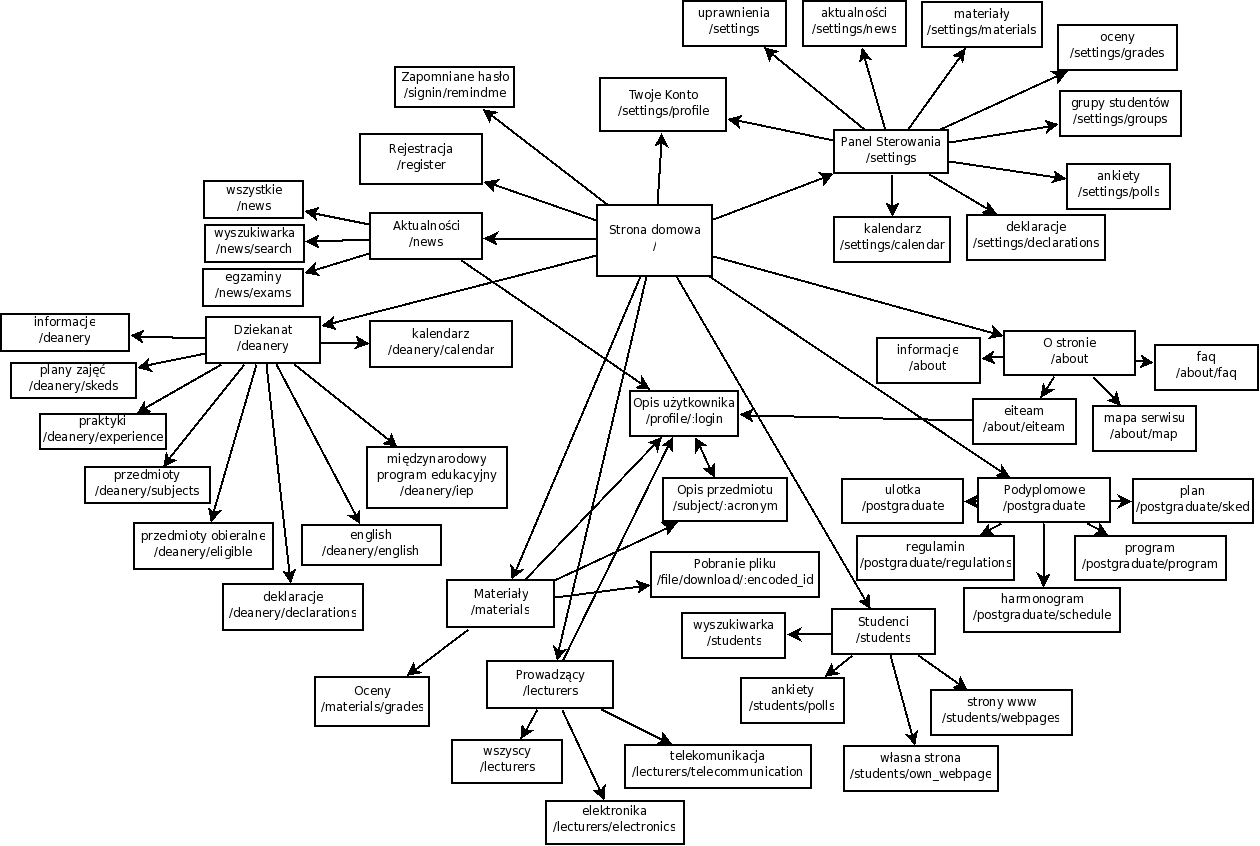
\includegraphics{mapa_eit.png}
  \caption{
  Mapa strony kierunku Elektronika i Telekomunikacja.
  \label{fig:eitmap}
  }
\end{figure}
\end{landscape}
\newpage
\addtolength{\textwidth}{-4cm}
\addtolength{\hoffset}{2.5cm}
\addtolength{\textheight}{-5cm}
\addtolength{\voffset}{3.5cm}



\section{Opis poszczególnych kontrolerów i akcji}
\label{sec:kontrolery}

\subsection{\emph{IndexController}}
\label{con:index}
  Główny kontroler, uruchamiany przy pierwszym wejściu na stronę.
\begin{itemize}
  \item \emph{index} -- akcja odpowiedzialna za wyświetlanie pierwszej, ,,zbiorczej'' strony EiT. Ładuje siedem ostatnich aktualności, siedem ostatnio dodanych materiałów, ostatnie ankiety oraz ostatnio dodane oceny. 
\end{itemize}

\subsection{\emph{AboutController}}
\label{con:about}
  Kontroler wyświetlający informacje o samej stronie EiT i ludziach, którzy ją tworzyli.
\begin{itemize}
  \item \emph{index} -- rys historyczny powstawania strony Elektroniki i Telekomunikacji,
  \item \emph{eiteam} -- ludzie odpowiedzialni za stronę,
  \item \emph{map} -- mapa serwisu
  \item \emph{faq} -- najczęściej zadawane pytania odnośnie witryny
\end{itemize}

\subsection{\emph{CsvController}}
\label{con:csv}
  Kontroler odpowiedzialny za generowanie plików \emph{.csv} i wysyłanie ich użytkownikom. Głównie stosowany, przy podsumowaniach deklaracji. Każda akcja wysyła określony plik csv.
\begin{itemize}
  \item \emph{language} -- informacje o językach prowadzenia przedmiotów, wybranych przez poszczególnych studentów,
  \item \emph{print} -- informacje o zainteresowaniu wydrukiem materiałów
  \item \emph{module} -- kto wybrał jaki moduł
  \item \emph{subjects} -- przypisanie studentów, do poszczególnych przedmiotów obieralnych
  \item \emph{experience} -- zbiorcze deklaracje praktyk
  \item \emph{speciality} -- informacje o wyborze kierunku studiów i specjalności
\end{itemize}

\subsection{\emph{DeaneryController}}
\label{con:deanery}
  Kontroler odpowiedzialny za wyświetlanie informacji z dziekanatu.
\begin{itemize}
  \item \emph{index} -- wyświetla podstawowe informacje o osobach pracujących w dziekanacie i godzinach przyjęć.
  \item \emph{skeds} -- lista planów zajęć do pobrania, w formacie XLS.
  \item \emph{experience} -- informacje dotyczące praktyk zawodowów na III i IV roku.
  \item \emph{subjects} -- lista wszystkich przedmiotów z podziałem na lata, kierunki i moduły. 
  \item \emph{eligible} -- lista przedmiotów obieralnych dla poszczególnych modułów i semestrów, wraz z liczbą studentów, którzy je wybrali.
  \item \emph{english} -- informacje o przedmiotach prowadzonych w języku angielskim.
  \item \emph{iep} -- informacje o międzynarodowym programie edukacyjnym.
  \item \emph{declarations} -- sekcja wymagająca zalogowania się. Dostępna tylko dla studentów. Umożliwia wszystkich aktualnie dostępnych deklaracji a także zawiera informacje na ich temat. Więcej informacji w sekcji ,,Deklaracje'' rozdz.~\ref{sub:deklaracje}, str.~\pageref{sub:deklaracje}.
  \item \emph{calendar} -- kalendarz studenta. Wszystkie istotne wydarzenia z punktu widzenia studenta (sesje, ferie, terminy składania podań, etc.).
\end{itemize}

\subsection{\emph{FileController}}
\label{con:file}
  Kontroler odpowiedzialny za pobieranie plików z serwisu.
\begin{itemize}
  \item \emph{download} -- zgodnie z polityką bezpieczeństwa, wszystkie pliki dodawane przez użytkowników, nie są trzymane w katalogu widocznym z poziomu serwera WWW. Bierze się to stąd, że wtedy każdy mógłby podać bezpośredniego linka do takiego pliku i cały mechanizm logowania i zabezpieczania materiałów byłby niepotrzebny. Zamiast tego, pliki leżą w specjalnym katalogu (tu \emph{/files}) i są przerabiane przez skrypt. Przerabianie to polega na sprawdzeniu czy plik istnieje, oraz czy użytkownik, który się do niego odwołuje ma do niego prawa dostępu. Jeśli tak, następuje pobranie, jeśli nie, strona zwraca błąd braku uprawnień.
\end{itemize}

\subsection{\emph{LecturersController}}
\label{con:lecturers}
  Kontroler wyświetlający informacje o wszystkich prowadzących dopisanych do systemu.
\begin{itemize}
  \item \emph{index} -- wyświetla listę wszystkich prowadzących, wraz z linkami do ich profili.
  \item \emph{electronics} -- j.w., ale tylko prowadzący Elektroniki
  \item \emph{telecommunication} -- j.w., ale tylko prowadzący Telekomunikacji
\end{itemize}

\subsection{\emph{MaterialsController}}
\label{con:materials}
  Kontroler odpowiedzialny za wyświetlanie i wyszukiwanie materiałów i ocen dodanych do serwisu.
\begin{itemize}
  \item \emph{index} -- wyświetla 10 ostatnich materiałów, oraz stanowi punkt wyjścia przy wyszukiwaniu kolejnych. Kiedy użytkownik wypełni pola i uruchomi wyszukiwanie, akcja ta pobiera zapytanie POST w formularza i przetwarza je na zapytanie GET. W takiej postaci przesyłane jest ono do akcji \emph{search}. Całe to przetwanie zrobione jest po to, aby można było również podawać zapytania do wyszukiwarki bezpośrednio w postaci linków -- w wielu miejscach, są np. linki do materiałów konkretnego prowadzącego, które nie są niczym innym jak odpowiednio spreparowanym zapytaniem dla akcji \emph{search}.
  \item \emph{search} -- pobiera zapytanie, stanowiące pięć kryteriów oddzielonych przecinkami. Są to kolejno:
  \begin{itemize}
    \item zakodowane ID przedmiotu
    \item zakodowane ID prowadzącego
    \item numer semestru
    \item treść wyszukiwania
    \item rodzaj sortowania wyników
  \end{itemize}
  w przypadku braku którejkolwiek z wartości, nie jest ona brana pod uwagę przy wyszukiwaniu.
  \item \emph{grades} -- dostępne tylko dla zalogowanych użytkowników listy ocen. Kryterium wyszukiwania jest grupa -- jeśli użytkownik i plik z oceną należą do tej samej, to link do pliku jest wyświetlany.
\end{itemize}

\subsection{\emph{NewsController}}
\label{con:news}
  Kontroler odpowiadający za wyświetlanie aktualności.
\begin{itemize}
  \item \emph{index} -- akcja wyświetlająca wszystkie aktualności (stronami, po 10) a także robiąca za przekaźnik wyszukiwarki (patrz niżej). 
  \item \emph{search} -- wyszukiwarka aktualności. Przyjmuje parametry rozdzielone przecinkami, przez GET. W przypadku ich braku wyświetla formularz. Mechanizm działania jest następujący -- użytkownik wpisuje szukaną informacje i określa kryteria wyszukiwania; następnie całość jest składana w zapytanie typu POST i zostaje przekierowane do akcji index; akcja index rozpakowuje zapytanie, buduje odpowiedni request GET dla akcji search a następnie wysyła go do akcji search; akcja search wyświetla posegregowana wyniki wyszukiwania (stronami, po 10).
  \item \emph{read} -- akcja, która jako parametr przyjmuje zakodowane ID wiadomości (zob. rozdz.~\ref{sub:idencoder}, str.~\pageref{sub:idencoder}), odkodowuje je, a następnie wyświetla aktualność o tym numerze.
  \item \emph{exams} -- akcja wyświetlające informacje o egzaminach w aktualnej sesji. Dodatkowo, jeżeli użytkownik posiada stosowne uprawnienia, umożliwia dodawanie, edycję i usuwanie egzaminów. 
\end{itemize}

\subsection{\emph{PostgraduateController}}
\label{con:postgraduate}
  Kontroler odpowiadający za wyświetlanie informacji na temat studiów podyplomowych.
\begin{itemize}
  \item \emph{index} -- ulotka reklamowa,
  \item \emph{regulations} -- regulamin,
  \item \emph{schedule} -- harmonogram,
  \item \emph{program} -- program,
  \item \emph{sked} -- plan zajęć.
\end{itemize}

\subsection{\emph{ProfileController}}
\label{con:profile}
  Kontroler odpowiedzialny za wyświetlanie informacji o użytkownikach.
\begin{itemize}
  \item \emph{view} -- wyświetla informacje o użytkowniku, którego zakodowane ID przyjmuje jako parametr. Zalogowany użytkownik może wyświetlić informacje o każdym, niezalogowany -- tylko o prowadzących.
\end{itemize}

\subsection{\emph{RedirectController}}
\label{con:redirect}
  Kontroler odpowiedzialny za odpowiednie przekierowywanie ze starych linków na nowe (zob. rozdz.~\ref{sec:mapa-linkow}, str.~\pageref{sec:mapa-linkow})
\begin{itemize}
  \item \emph{index} -- przekierowuje na adres podany w parametrze
\end{itemize}

\subsection{\emph{RegisterController}}
\label{con:register}
  Kontroler odpowiedzialny za rejestrację. Cały mechanizm rejestracji jest dość specyficzny, z racji tego, że nie każdy może dołączyć do serwisu. Dopisać się mogą tylko ludzie, znajdujący się na liście studentów corocznie dostarczanej przez dziekanat. Takie osoby są dopisywane do bazy, bez przydzielonego logina i hasła. Proces rejestracj polega więc, wpierw na uwierzytelnieniu się swoim imieniem, nazwiskiem i numerem indeksu, a następnie na podaniu pozostałych informacji o sobie. Po pomyślnym jego przejściu, student staje się użytkownikiem systemu.
\begin{itemize}
  \item \emph{index} -- przeprowadzenie procesu rejestracji, tylko dla niezalogowanych użytkowników.
\end{itemize}

\subsection{\emph{RssController}}
\label{con:rss}
  Kontroler generujący treść dla czytników RSS (zob. rozdz.~\ref{sec:rss}, str.~\pageref{sec:rss}).

\begin{itemize}
  \item \emph{index} -- zwraca 15 ostatnich aktualności w formacie zgodnym z RSS.
\end{itemize}

\subsection{\emph{RtfController}}
\label{con:rtf}
  Kontroler stworzony w celu serwowania predefiniowanych, dynamicznie uzupełnianych dokumentów \emph{.rtf}.
\begin{itemize}
  \item \emph{experience} -- wysyła użytkownikowi (oczywiście, jeśli ma odpowiednie uprawnienia), komplet gotowych umów o praktykę, między studentami (którzy wypełnili deklaracje praktyk) a ich zakładami pracy.
\end{itemize}

\subsection{\emph{SettingsController}}
\label{con:settings}
  Kontroler zbiorczy, odpowiedzialny za wszystkie zadania związane z administracją serwisu.
\begin{itemize}
  \item \emph{index} -- wyświetlenie strony powitalnej, zawierającej odnośniki do wszystkich sekcji administracyjnych wraz z określeniem praw dostępu (zielona kropka -- dostęp dozwolony, czerwona -- zabroniony).
  \item \emph{news} -- administracja aktualnościami
  \item \emph{materials} -- dodawanie materiałów oraz ustalanie do nich praw dostępu
  \item \emph{grades} -- j.w. tyle, że oceny
  \item \emph{groups} -- administrowanie grupami studentów. Nie można zmienić domyślnie zadeklarowanych, można jednak dodawać, usuwać i edytować swoje.
  \item \emph{polls} -- dodawanie ankiet. W systemie mogą być maksymalnie dwie -- jedna anonimowa i jedna nie, dodanie każdej nowej spowoduje zamknięcie poprzedniej.
  \item \emph{declarations} -- wyświetlenie informacji o deklaracjach wypełnionych przez studentów oraz zarządzanie nimi (zob. rozdz.~\ref{sub:deklaracje}, str.~\pageref{sub:deklaracje}.
  \item \emph{calendar} -- zarządzanie kalendarzem studenta
  \item \emph{profile} -- zarządzanie profilem aktualnie zalogowanego użytkownika. Z poziomu tej akcji, można zmienić swój login, hasło i kilka innych danych.
\end{itemize}

\subsection{\emph{SigninController}}
\label{con:signin}
  Kontroler obsługujący wszelkie akcje związane z logowaniem użytkownika do systemu.
\begin{itemize}
  \item \emph{index} -- akcja odpowiadająca za logowanie użytkownika,
  \item \emph{signout} -- wylogowuje zalogowanego,
  \item \emph{remindme} -- uruchamia procedure odzyskania zapomnianego hasła. Wpierw użytkownik proszony jest o podanie imienia, nazwiska i numeru indeksu. Jeżeli dane te zostaną pomyślnie zweryfikowane użytkownikowi wyświetlone jest pytanie kontrolne. Odpowiedź na nie, jest przekierowywana do akcji \emph{answer}. W przypadku, kiedy użytkownik nie zadeklarował pytania ratunkowego, wyświetlana jest stosowna informacja.
  \item \emph{answer} -- ta akcja sprawdza odpowiedź podaną przez użytkownika na pytanie kontrolne. Jeśli jest poprawna, następuje zalogowanie do systemu.
\end{itemize}

\subsection{\emph{StudentsController}}
\label{con:students}
  Kontroler zawierający wszelkie informacje dotyczące samych studentów.
\begin{itemize}
  \item \emph{index} -- wyszukiwarka studentów, dostępna tylko dla zalogowanych użytkowników. Pozwala na wybór kryteriów wyszukiwania, wpływ na wyświetlane wyniki i określenie kolumny po której odbędzie się końcowe sortowanie. Całe zapytanie POST z formularza jest przesyłane do akcji \emph{results}.
  \item \emph{results} -- przetwarza zapytanie POST z wyszukiwarki i wyświetla pasujące do kryteriów wyszukiwania wyniki, odpowiednio posortowane i opisane.
  \item \emph{own\_webpage} -- informacje dla studentów chcących sobie założyć własną stronę WWW na serwerach EiT.
  \item \emph{webpages} -- lista wszystkich stron WWW na serwerze EiT. Lista jest tworzona, poprzez przeszukanie wszystkich katalogów domowych użytkowników pod kątem katalogu \emph{public\_html}. Wszyscy użytkownicy, którzy mają taki katalog a ich loginy, zgadzają się z loginami w bazie zostają wyświetleni. Dodatkowo, w rubryce ,,Opis strony domowej'' pojawia się zawartość pliku \emph{.webinfo} znajdującego się w katalogu ze stroną (o ile istnieje).
\end{itemize}

\subsection{\emph{SubjectController}}
\label{con:subject}
  Kontroler wyświetlający informacje o przedmiocie.
\begin{itemize}
  \item \emph{method\_missing} -- jest to specjalna metoda w Rubym. Jest ona zawsze wywoływana, gdy obiekt próbuje odwołać się do nieistniejącej metody. Jako pierwszy parametr, przyjmuje jej nazwę. W tym przypadku, nazwa ta jest interpretowana jako akronim nazwy przedmiotu i jeśli zostanie odnaleziony w bazie, wszelkie informacje na temat tych zajęć są wyświetlane użytkownikowi.
\end{itemize}

\section{Komponenty}
\label{sec:components}
  Aby aplikacja działała poprawnie, niezbędne okazało się stworzenie kilku komponentół -- małych klas, stworzonych w jednym, skonkretyzowanym celu. Dzięki temu, zgodnie z regułą DRY (zob. rozdz.~\ref{sec:dry}, str.~\pageref{sec:dry}), wszystko jest w jednym miejscu.
\subsection{IdEncoder}
\label{sub:idencoder}
  IdEncoder to klasa krytyczna z punktu widzenia bezpieczeństwa aplikacji. Jej zadaniem jest kodowanie cyfr (zazwyczaj numerów \emph{id} wierszy, stąd nazwa \emph{IdEncoder}) na trudny do złamania ciąg znaków. Głównym celem takiego postępowania jest zabezpieczenie się przed wszelkiego rodzaju botami, które chodząc po stronie mogłyby inkrementować liczniki co 1 i w ten sposób powyciągać wszystkie informacje z bazy. Dodatkowo zabezpiecza to przed ,,sprytnymi'' użytkownikami, którzy mając dostęp do materiału o id np. 3, a nie mając do 4, próbowaliby podmieniać cyfry w adresach URL. Po instalacji aplikacji, należy w klasie IdEncoder ustawić dwie zmienne:
\begin{itemize}
  \item \emph{hash} -- jest to liczba z zakresu <0;4294967295>, z którą id będzie poddane opearacji ExOR na początku kodowania,
  \item \emph{salt} -- jest to dwudziestocyfrowa liczba, z której 10 cyfr będzie użyte do zaciemnienia wyniku w końcowym etapie kodowania.
\end{itemize}
Schemat kodowania jest następujący:
\begin{equation}
  id_{XOR} = id \oplus hash
\end{equation}
\begin{equation}
  salt_{M} = salt_{MARKER} = id_{XOR}~mod~10
\end{equation}
\begin{equation}
  id_{ENC} = \left(\frac{salt~mod~10^{20 - salt_{M}} - salt~mod~10^{20 - salt_{M} - 10}}{10^{20 - salt_{M} - 10}} * 10 + salt_{M}\right)_{(28)}
  \label{equ:idenc}
\end{equation}
Rozkodowywanie odbywa się w analogiczny sposób, tylko w drugę stronę.

Dodatkowo, algorytm został tak pomyślany, że nawet znając schemat postępowania niemożliwe jest rozkodowanie liczby, bez znajomości \emph{hash} i \emph{salt}.

Użycie klasy jest bardzo proste:
\begin{figure}[h]
\begin{verbatim}IdEncoder.encode(id)         # zakoduj id
IdEncoder.decode(encoded_id) # zdekoduj id\end{verbatim}
\caption{Użycie polecenia IdEncoder\label{fig:idenc}}
\end{figure}

\subsection{Pager}
\label{sub:pager}
Klasa \emph{Pager} jest wykorzystywana wszędzie tam, gdzie zwracana ilość wyników jest zbyt duża i umieszczenie ich na jednej stronie znacznie zmniejszyłoby czytelność, lub wręcz ją uniemożliwiło (wygenerowana strona byłaby tak duża, że ściągnięcie jej zajęłoby zbyt dużo czasu). Konstrukcja konstruktora jest następująca:

\begin{figure}[h]
\begin{verbatim}def initialize params, results, params_key = :id, actual_page = nil,
               results_per_page = 10\end{verbatim}
\caption{Struktura konstruktora klasy Page\label{fig:page}}
\end{figure}


Gdzie parametry to:
\begin{itemize}
  \item \emph{params} -- tablica params z kontrolera. Z racji tego, że komponenty są oddzielone od warstwy aplikacji, nie widzą domyślnych tablic Ruby~on~Rails (m.in. params), dlatego należy je przekazać. Jest to konieczne, aby Pager mógł poprawnie budować odnośniki.
  \item \emph{results} -- zawiera obiekt modelu danych wyciągniętych bezpośrednio z bazy, które mają być podzielone na strony.
  \item \emph{params\_key} -- domyślnie \emph{:id}. Określa który parametr routera Rails, ma być interpretowany jako numer kolejnej strony z wynikami (czasami zdarza się, że \emph{:id} jest już wykorzystane do czegoś innego, wtedy ta opcja się przydaje).
  \item \emph{actual\_page} -- wymuszenie zwrócenia wyników dla określonej strony. Domyślnie, brana jest strona z params[params\_key] (lub pierwsza, jeśli podana wartość jest błędna lub nieistniejąca).
  \item \emph{results\_per\_page} -- określa ile wyników ma być zareprezentowanych na jednej stronie. Domyślnie jest to 10.
\end{itemize}
Dodatkowo Pager zawiera wiele przydatnych metod, użytecznych przy budowaniu widoków. Są to:
\begin{itemize}
  \item \emph{count} -- zwraca ilość stron,
  \item \emph{array\_of\_pages} -- zwraca pasek nawigacyjny Pagera. To te cyfry z numerami stron i strzałkami ,,poprzednia'', ,,następna'' etc. (zobacz rysunek \ref{fig:array_of_pages}). Przyjmuje dwa parametry:
  \begin{itemize}
    \item \emph{page\_number} -- względem której strony ma być wyskalowany. Domyślnie jest to aktualna strona.
    \item \emph{pages\_padding} -- odnośniki do ilu stron wokół aktywnej, mają zostać wyświetlone. Domyślnie trzy.
  \end{itemize}
  \item \emph{last\_page} -- zwraca numer ostatniej strony,
  \item \emph{results} -- zwraca wyniki w zakresie odpowiednim dla aktualnej strony,
  \item \emph{all\_results} -- zwraca wszystkie wyniki (czyli tak naprawdę obiekt \emph{results} przekazany do konstruktora),
  \item \emph{results\_count} -- zwraca liczbę wszystkich wyników,
  \item \emph{results\_range} -- zwraca pełny zakres dostępnych stron oddzielonych separatorem przekazanym jako parametr. Czyli np. ,,1 - 123'', zobacz rysunek \ref{fig:array_of_pages}
  \item \emph{actual\_page} -- zwraca numer aktualnej strony
  \item \emph{next\_page} -- zwraca numer następnej strony
  \item \emph{previous\_page} -- zwraca numer poprzedniej strony
\end{itemize}
\begin{figure}[h]
\centering
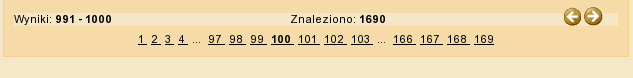
\includegraphics{array_of_pages.png}
\caption{Ilustracja wykorzystania \emph{array\_of\_pages}, gdzie \emph{page\_number} = 100, a \emph{pages\_padding} = 3\label{fing:array_of_pages}. Dodatkowo na górze po lewej, efekt działania \emph{results\_range} z domyślnym separatorem}
\end{figure}

Dodatkowo Pager ma przygotowany, predefiniowany dla serwisu EiT widok wyświetlający nawigację, który można znaleźć w \emph{app/views/\_partials/\_pager.rhtml}.

\subsection{Imieniny}
\label{sub:nameday}
Klasa \emph{NameDay} to bardzo prosta, statyczna klasa o jednej metodzie -- \emph{get}. Przyjmuje ona dwa parametry: dzień i miesiąc, a następnie zwraca gotowy łancuch znaków zawierający oddzielone przecinkiem imieniny osób w tym dniu.

\subsection{Deklaracje}
\label{sub:deklaracje}
System deklaracji to najdynamiczniej zmieniająca się część serwisu. Niektóre deklaracje stają się przestarzałe, czasami dochodzą nowe. Projektując system deklaracji, od początku trzeba było mieć to na uwadze. Oznacza to, że deklaracji nie można było po prostu ,,zaszyć'' w kontrolerze. Dlatego też autor wybrał inne rozwiązanie -- system deklaracji, jako system wtyczek. Każdy rodzaj deklaracji ma swój własny oddzielny plugin. Dzięki temu, łatwo w przyszłości będzie dodawać nowe deklaracje, bez naruszenia integralności serwisu. 

\subsubsection{Pliki}
\label{subsub:dec-files}
Pliki do systemu deklaracji znajdują się w trzech miejscach:
\begin{itemize}
  \item \emph{components/declarations/} -- tutaj znajdują się klasy deklaracji. Każdy rodzaj deklaracji, ma swoją oddzielną klasę. Więcej szczegółów odnośnie klas, znajduje się w dalszej części tego rozdziału.
  \item \emph{app/views/deanery/declarations/} -- widoki deklaracji, przeznaczone dla studentów. To właśnie one są wyświetlane, w momencie kiedy student wypełnia deklarację. Należy trzymać się konwencji \emph{nazwa deklaracji}$\to$\emph{nazwa widoku}. Jeśli widoków dla jednej deklaracji będzie więcej, informację identyfikującą należy dodawać po twardej spacji.
  \item \emph{app/views/settings/declarations/} -- analogicznie jak powyżej, tyle że widoki przeznaczone są dla prowadzących mających dostęp do ustawień deklaracji.
\end{itemize}

\subsubsection{Klasa główna}
Wszystkie klasy deklaracji powinny dziedziczyć z klasy \emph{Declarations}, która znajduje się w \emph{components/declarations.rb}. Klasa ta, dostarcza klasom potomnym nastęþujące zmienne klasy:
\begin{itemize}
  \item \emph{@logged\_user} -- obiekt zalogowanego użytkownika
  \item \emph{@declarations\_subjects} -- obiekt modelu DeclarationsSubject (tabela \emph{declarations\_subjects}, zob. rozdz.~\ref{subsub:declarations_subjects}, str.~\pageref{subsub:declarations_subjects}) zawierający tylko przedmioty dotyczące deklaracji potomnej
  \item \emph{@merged\_subjects} -- początkowo pusta. Domyślnie powinna zawierać przedmioty podane w deklaracji przez użytkownika (jeżeli jest to konieczne). Wcześniej należy przepuścić je przez specjalny skrypt, który usuwa wszystkie podejrzane lub błędne wpisy (zabezpieczenie przed fałszerstwem) -- skrypt ten, to \emph{merge\_subjects}
  \item \emph{@flash\_notice} -- wiadomość, jaka ma zostać wyświetlona w czasie wypełniania deklaracji. Domyślnie jest pusta, ale nic nie stoi, aby klasa potomna ją ustawiła w razie potrzeby.
  \item \emph{@template} -- nazwa widoku, który ma zostać wyrenderowany. Aplikacja sama dobierze ścieżkę.
  \item \emph{@declaration\_name} -- nazwa deklaracji (pole \emph{head} w tabeli \emph{declarations}, zob. rozdz.~\ref{subsub:declarations}, str.~\pageref{subsub:declarations})
  \item \emph{@declaration\_id} -- numer \emph{id} deklaracji
\end{itemize}

\subsubsection{Klasy potomne}
Każda klasa potomna powinna mieć dwie metody -- \emph{execute} oraz \emph{setup}. Obie powinny przyjmować jeden parametr -- będzie to \emph{params} z Ruby~on~Rails. Metoda execute wywołuje się w kontrolerze \emph{DeaneryController}, jest więc przeznaczona dla studentów wypełniających deklaracje. Metoda \emph{setup} wywoła się w kontrolerze \emph{SettingsController}, jest więc przeznaczona dla prowadzących zarządzających deklaracjami. Najważniejsze o czym należy pamiętać w klasach potomnych, to ustawianie zmiennej \emph{@template} z odpowiednim widokiem oraz o tym, aby później inicjalizacje klas potomnych dopisać do metod \emph{declarations} w wyżej wymienionych kontrolerach.

\subsubsection{Struktura bazy danych i relacji}
Wszystkie informacje odnośnie deklaracji po stronie bazy danych zostały opisane w:
\begin{itemize}
  \item Rozdz.~\ref{sub:tabele}, str.~\pageref{subsub:declarations} (Tabela \emph{declarations})
  \item Rozdz.~\ref{sub:tabele}, str.~\pageref{subsub:declarations_subjects} (Tabela \emph{declarations\_subjects})
  \item Rozdz.~\ref{sub:relacje}, str.~\pageref{subsub:declarations-declarations_subjects}
\end{itemize}

Po utworzeniu nowego plugina należy dopisać odpowiednie deklaracje do tabeli \emph{declarations}, oraz ewentualnie utworzyć nowe kolumny w tabeli \emph{declarations\_columns} i wypełnić je danymi początkowymi.

\section{Przemapowanie hiperłączy}
\label{sec:mapa-linkow}
Ostatnim problemem jaki należało rozwiązać był problem linków. Nowa aplikacja posiada zupełnie inaczej rozwiązany system odnośników. Nie są to już trzyliterowe, nic nie mówiące skróty, tylko pełne nazwy angielskie. Takie podejście ułatwia pracę robotom wsyszukiwarek, pozycjonuje wyżej stronę, ułatwia ludziom zapamiętanie linka i przygotowuje grunt pod przyszłe tłumaczenie serwisu. Niestety na chwilę obecną, cała strona EiT jest zaindeksowana pod starymi adresami i wrzucenie nowej aplikacji zakończyłoby się ogromną ilością martwych linków. Użytkownik wyszukiwarki po kliknięciu na takie hiperłącze zostałby oddelegowany w próżnię. Aby tego uniknąć stworzony został mapper do linków. Jest to po prostu zestaw regułek w pliku \emph{config/routes.rb}, który tłumaczy stare linki na nowe.

Niestety same wpisy w \emph{routes.rb} nie wystarczą, gdyż wtedy skończylbyśmy z nową treścią renderowaną pod starym adresem URL. Nie jest to zachowanie oczekiwane, gdyż w ten sposób stare linki nigdy nie zniknęłyby z wyszukiwarek. Dlatego trzeba jeszcze dodać przekierowanie -- czyli zastosować kod HTTP~301 \emph{Moved permanently}. Niestety system routingu w Ruby~on~Rails nie przewiduje takiego zastosowania, dlatego trzeba posłużyć się pewnym obejściem. Mianowicie, wszystkie zapytania o stare linki są wpierw kierowane do kontrolera \emph{RedirectController}, a jako parametr podawany jest nowy adres. Kontroler ten, wysyła następnie kod 301 i przekierowuje użytkownika na odpowiednią stronę.

Rozwiązanie takie ma dwie zalety. Po pierwsze, użytkownik klikając w wyszukiwarce na odnośnik, znajduje się już na nowej stronie i od razu widzi w pasku adresu nowy link, dzięki temu nie przywiązuje się do starych oznaczeń. Po drugie, wyszukiwarki dużo szybciej usuwają stare linki i przeindeksowują je sobie na nowe, jeśli napotykają kod \emph{Moved Permamently}.

\section{Testowanie i instalacja}
\label{sec:testowanie}
Cześć implementacji projektu została zakończona. Ruby~on~Rails posiada także wbudowaną funkcjonalność pozwalającą na kompleksowe testowanie aplikacji. Zarówno na poziomie jednostkowym, jak i funkcjonalnym. Nie da się ukryć że tworzenie testów bardzo pomaga w rozwoju aplikacji i chociaż jest bardzo pracochłonne w dłuższej perspektywie pozwala zaoszczędzić czas. Jednak aplikacja opisana w pracy na chwilę obecną jest mała a całość kodu został napisana przez jednego programistę. Dopisanie testów zajęło by kilka dobrych dni. Autor jest w stanie samodzielnie kompleksowo ją przetestować, dlatego zrezygnował z pisania testów.
Instalacja i uruchomienie ogranicza się do przekopiowania całości kodu na docelowy serwer, który będzie posiadał wszystkie niezbędne komponenty (wymienione w podrozdziale Przygotowanie środowiska pracy, zob. str.~\pageref{sec:srodowisko}). Następnie wystarczy skonfigurować odpowiednie połączenia z bazami w pliku \emph{config/database.yml} (zob. rozdz.~\ref{sub:convert-base}, str.~\pageref{sub:convert-base}), przygotować strukturę w nowej bazie danych (uruchamiając polecenie \verb+rake db:migrate+) i przekonwertować starą bazę na nową (polecenie \verb+rake eit:db:convert+). Potem już tylko wystarczy uruchomić serwer i gotowe.
\begin{figure}[h]
\centering
\begin{verbatim}rake db:migrate
rake eit:db:convert
mongrel_rails start -p 80 -l ./log/mongrel.log -e production)\end{verbatim}
\caption{Kompletny zestaw poleceń, niezbędny do uruchomienia aplikacji\label{fig:runapp}}
\end{figure}

\chapter{Zakończenie}
\label{cha:end}


\end{document}
